% =============================================================================
% main.tex — Zero-Shot Text Classification with Locally-Hosted Large Language Models
% Authors: Luigi Palumbo, Mengting Yu
% =============================================================================
\documentclass[11pt,a4paper]{article}

% ---------- Packages ----------
\usepackage[utf8]{inputenc}
\usepackage[T1]{fontenc}
\usepackage{lmodern}
\usepackage[margin=2.5cm]{geometry}
\usepackage{booktabs}
\usepackage{graphicx}
\graphicspath{{experiment/}}
\usepackage{hyperref}
\usepackage{xcolor}
\usepackage{listings}
\usepackage{enumitem}
\usepackage{caption}
\usepackage{subcaption}
\usepackage{float}
\usepackage{amsmath,amssymb}
\usepackage{siunitx}
\usepackage{microtype}
% Give justified text last-resort stretch so long unbreakable tokens
% (e.g.\ \texttt{::}-paths) do not produce overfull boxes.
\setlength{\emergencystretch}{3em}

% Placeholder for "not applicable" cells in tables.
\providecommand{\dm}{---}

% ---------- Bibliography ----------
\usepackage[style=apa,backend=biber,natbib=true]{biblatex}
\addbibresource{references.bib}

% Suppress internal annote/annotation fields from bibliography display
\AtEveryBibitem{%
  \clearfield{annotation}%
  \clearfield{annote}%
}

% ---------- Hyperref setup ----------
\hypersetup{
  colorlinks=true,
  linkcolor=blue!70!black,
  citecolor=blue!70!black,
  urlcolor=blue!60!black,
}

% ---------- Listings setup ----------
\lstset{
  language=Python,
  basicstyle=\ttfamily\small,
  keywordstyle=\color{blue!70!black}\bfseries,
  commentstyle=\color{green!50!black}\itshape,
  stringstyle=\color{red!70!black},
  breaklines=true,
  frame=single,
  numbers=left,
  numberstyle=\tiny\color{gray},
  backgroundcolor=\color{gray!5},
}

% ---------- Additional listings languages (R, Rust) ----------
\lstdefinelanguage{R}{%
  morekeywords={if,else,for,while,repeat,function,return,in,TRUE,FALSE,
    NULL,NA,Inf,NaN,library,require},
  sensitive=true,
  morecomment=[l]{\#},
  morestring=[b]",
  morestring=[b]',
}
\lstdefinelanguage{Rust}{%
  morekeywords={fn,let,mut,pub,use,mod,struct,enum,impl,trait,return,if,
    else,for,while,loop,match,as,in,ref,move,where,async,await,dyn,unsafe,
    const,static,Self,self,super,crate,true,false,None,Some,Ok,Err,vec},
  sensitive=true,
  morecomment=[l]{//},
  morecomment=[s]{/*}{*/},
  morestring=[b]",
}

% ---------- Title ----------
\title{
  \textbf{Zero-Shot Text Classification with Locally-Hosted\\
  Large Language Models: The \texttt{ollama-classifier} Library}
}
\author{
  Luigi Palumbo\thanks{Bank of Italy. Corresponding author.}
  \and Mengting Yu\thanks{Università degli Studi della Tuscia.}
}
\date{\today}

% =============================================================================
\begin{document}

\maketitle

% ---------- Abstract ----------
\begin{abstract}
  Large Language Models (LLMs) are powerful zero-shot classifiers, yet their
  adoption in domains that demand data privacy, cost control, and offline
  operation remains limited by reliance on proprietary cloud
  application-programming interfaces (APIs). We present
  \texttt{ollama-classifier}, an open-source Python library for zero-shot and
  few-shot text classification with locally-hosted LLMs. The library exposes
  two complementary scoring strategies---multi-call completion scoring
  (\texttt{classify}) and hierarchical constrained generation
  (\texttt{generate})---both yielding a full probability distribution and a
  confidence score; \texttt{generate} does so in a single call, with optional
  mass-preserving refinement. Both are available across four inference
  backends (Ollama, vLLM, SGLang, llama.cpp) through a unified interface. A
  no-code desktop graphical user interface (GUI)
  (\texttt{ollama-classifier-gui}) and cross-language
  ports in R (\texttt{rollama}) and Rust
  (\texttt{ollama-classifier-rs}) extend the same API to non-programmers and
  to other language ecosystems. We benchmark the library against
  BART-large-MNLI and scikit-llm on a COICOP (Classification of Individual
  Consumption According to Purpose) product-classification task and
  show that a compact 3B-parameter model served locally substantially
  outperforms the natural-language-inference (NLI) baseline and matches scikit-llm in accuracy, while
  additionally providing confidence scores---and the margin between the two
  highest class probabilities---that reliably discriminate correct from
  incorrect predictions and support threshold-based triage.
\end{abstract}

\noindent\textbf{Keywords:} zero-shot classification, large language models,
local inference, constrained generation, confidence calibration, Ollama,
open-source software

% =============================================================================
\section{Introduction}
\label{sec:introduction}
% =============================================================================

The advent of Large Language Models (LLMs) has transformed natural language
processing, enabling zero-shot and few-shot performance across a wide range
of tasks \citep{brown2020language, radford2019gpt2, zhao2023survey}. Text
classification---the assignment of predefined labels to free-form text---is a
particularly impactful application, with use cases spanning sentiment analysis
\citep{wang2024sentiment}, economic-taxonomy coding, and product
categorization \citep{nunes2025rac}.

Traditional text classification relies on supervised pipelines that demand
labeled training data, feature engineering, and model fine-tuning.
Transformer encoders such as BERT \citep{berki2025nlp} improve accuracy but
remain data-intensive and adapt poorly to evolving taxonomies without costly
retraining. LLMs challenge this paradigm: models such as GPT-3
\citep{brown2020language} and GPT-4 \citep{openai2023gpt4} perform
classification through in-context learning, removing the need for
task-specific training data. Deploying these capabilities in production,
however, and especially in sensitive domains such as official statistics,
healthcare, or finance, raises three concerns: proprietary cloud APIs incur
recurring costs, require internet connectivity, and expose confidential or
regulated data to third parties.

The proliferation of open-source LLMs---LLaMA \citep{touvron2023llama,
meta2024llama3}, Mistral \citep{jiang2023mistral}, Qwen
\citep{yang2024qwen2}, and DeepSeek-R1 \citep{deepseek2025r1}---together with
lightweight serving frameworks such as Ollama \citep{ollama} makes capable
models runnable on consumer hardware. This creates an opportunity to build
classification tools that combine the zero-shot reasoning of LLMs with the
privacy, cost-effectiveness, and offline capability of local inference.

We present \texttt{ollama-classifier} \citep{ollama-classifier}, an
open-source Python library that realizes this opportunity through a unified
interface for zero-shot and few-shot text classification with locally-hosted
LLMs. The library is built around three principles:

\begin{enumerate}[leftmargin=*]
  \item \textbf{No fine-tuning required.} Classification uses prompting and
        retrieval augmentation, exploiting the model's pre-trained knowledge
        without task-specific training.
  \item \textbf{Local and private.} All inference runs on the user's hardware
        through Ollama or a compatible backend, so no data leaves the machine.
  \item \textbf{Accompanied by calibrated uncertainty.} Every prediction
        carries a full probability distribution and a confidence score,
        enabling triage between auto-accepted labels and items requiring
        human review.
\end{enumerate}

The remainder of the paper is organized as follows.
Section~\ref{sec:related} reviews related work; Section~\ref{sec:background}
covers the enabling technologies; Section~\ref{sec:library} describes the
library's API and confidence-scoring methodology; Section~\ref{sec:ecosystem}
presents the GUI and the cross-language ports; and
Section~\ref{sec:application} reports a benchmark evaluation on COICOP
product classification, including a calibration and threshold-discrimination
analysis. Section~\ref{sec:discussion} discusses design decisions and
limitations, and Section~\ref{sec:conclusion} concludes.

% =============================================================================
\section{Related Work}
\label{sec:related}
% =============================================================================

\subsection{LLMs as Classifiers}

Generative language models perform discriminative tasks through careful
prompt design. \citet{radford2019gpt2} first showed that GPT-2 could perform
zero-shot task transfer, and \citet{brown2020language} scaled the result with
GPT-3, where few-shot in-context learning reached competitive classification
accuracy without gradient updates. \citet{liu2023preliminary} survey prompting
methods, and \citet{mu2024prompt} show that well-structured prompts with
explicit output constraints materially improve zero-shot accuracy.
\citet{gilardi2023chatgpt} demonstrate that ChatGPT can match or exceed
crowd-worker quality on text annotation, supporting LLMs as practical
classifiers.

\subsection{Retrieval-Augmented Classification}

Retrieval-Augmented Generation \citep{lewis2020retrieval} grounds LLM outputs
in externally retrieved evidence, improving factuality and stability. Adapted
to classification as Retrieval-Augmented Classification (RAC),
\citet{yu2023retrieval} combine nearest-neighbor retrieval with few-shot
prompting, and \citet{abdullahi2024retrieval} extend the idea to the
zero-shot setting. Most relevant to this work, \citet{nunes2025rac} apply RAC
to COICOP 2018 product classification, building a synthetic knowledge base of
34{,}451 exemplars and reaching up to 0.80 accuracy at the finest taxonomy
level. \texttt{ollama-classifier} operationalizes the final part of this pipeline as a
general-purpose, reusable library.

\subsection{Existing Classification Libraries}

Several open-source projects address LLM-based classification.
\texttt{llmclassifier} \citep{cvxtz2023llmclassifier} and
\texttt{llmClassificR} \citep{golino2023llmclassificr} build classification
pipelines on top of API-hosted models. \texttt{scikit-llm}
\citep{ScikitLLM} offers a scikit-learn-compatible interface for zero-shot
and few-shot classification and can be pointed at a local model server
through an OpenAI-compatible endpoint. \texttt{scikit-ollama} \citep{skollama} extends the 
approach to Ollama-hosted models. Unlike \texttt{ollama-classifier},
scikit-llm and scikit-ollama are label-only classifiers: they return the predicted class but no
calibrated confidence scores or full probability distribution, which precludes
the uncertainty-aware triage workflows analyzed in
Section~\ref{sec:application}. \texttt{ollama-classifier} further
differentiates itself by focusing on local inference across multiple serving
engines, by enforcing constrained output generation, and by shipping a
dedicated GUI and cross-language ports (Section~\ref{sec:ecosystem}).

% =============================================================================
\section{Background}
\label{sec:background}
% =============================================================================

\subsection{Local LLM Serving and Inference Backends}

Ollama \citep{ollama} is an open-source runtime for running LLMs locally on
consumer hardware. It provides a lightweight model server with a
Representational State Transfer (REST) API,
model management (pull, list, delete), and quantized inference that allows
models from 1B to 70B+ parameters to run on standard workstations. The Ollama
Python library \citep{ollama_python} exposes this API and structured outputs;
\texttt{ollama-classifier} wraps it (and the equivalent clients of other
engines) behind a higher-level classification interface.

While Ollama is the default backend, \texttt{ollama-classifier} supports four
inference engines through a common interface: \emph{Ollama} for consumer
hardware and single-user workflows; \emph{vLLM} for high-throughput batch
inference; \emph{SGLang} for low-latency serving; and \emph{llama.cpp} for
resource-constrained central processing unit (CPU) and mixed
CPU/graphics processing unit (GPU) environments. All four expose the
per-token log-probabilities that the confidence-scoring methods require
(Section~\ref{sec:confidence}); they differ in how those log-probabilities
are obtained and in the constraint mechanism used to enforce valid labels.

% SUBSECTION REMOVED, NOT RELEVANT TO THE PAPER
% \subsection{Embedding Models for Retrieval}

% The retrieval stage of RAC relies on embedding models that map text to dense
% vectors. SentenceTransformers \citep{reimers2019sentence} provides the
% foundational Siamese-BERT architecture; the E5 family
% \citep{wang2022text} offers multilingual similarity across 100 languages; and
% the GTE family \citep{chen2024gte} provides instruction-tuned embeddings with
% strong multilingual performance. In the RAC evaluation of
% \citet{nunes2025rac}, GTE models achieved the highest retrieval presence
% (90.7\%), confirming their effectiveness for classification-oriented
% retrieval.

% =============================================================================
\section{The \texttt{ollama-classifier} Library}
\label{sec:library}
% =============================================================================

\subsection{Design Philosophy}

\texttt{ollama-classifier} is a lightweight, modular library that performs
text classification through a minimal API surface. Its design follows four
principles: \emph{simplicity}, since a classification call needs only a text
and a set of candidate labels, with all prompt construction, output parsing,
and backend communication handled internally; \emph{flexibility}, since users
can customize the system prompt, supply label descriptions, choose between
two scoring strategies, and switch backends transparently; \emph{reliability},
since constrained output generation forces valid labels and confidence scores
enable triage between auto-accepted and human-reviewed items; and
\emph{scalability}, since batch and asynchronous APIs process large datasets
with concurrent requests across all backends.

\subsection{Core API}

The library exposes a single backend-agnostic entry point,
\texttt{LLMClassifier}, constructed over a backend such as
\texttt{OllamaBackend}. Table~\ref{tab:api} summarizes its methods. Each
synchronous method has an asynchronous twin prefixed with \texttt{a}
(\texttt{agenerate}, \texttt{aclassify}, \dots), and both strategies have
batch variants.

\begin{table}[htbp]
  \centering
  \caption{Core methods of the \texttt{ollama-classifier} API.}
  \label{tab:api}
  \begin{tabular}{lp{8.2cm}}
    \toprule
    \textbf{Method} & \textbf{Description} \\
    \midrule
    \texttt{generate()} & Hierarchical constrained generation. A single
                          constrained call reconstructs a full probability
                          distribution from divergence-aware log-probabilities;
                          optional \texttt{max\_calls} refines it through
                          mass-preserving cluster reproportioning. \\
    \texttt{classify()} & Multi-call completion scoring. Makes one call per
                          candidate label and returns exact, calibrated
                          probabilities. \\
    \texttt{batch\_generate()} / \texttt{batch\_classify()} & Batch variants
                          for many texts. \\
    \bottomrule
  \end{tabular}
  % \footnotesize{Both \texttt{generate} and \texttt{classify} return a
  %   \texttt{ClassificationResult} carrying the prediction, a confidence
  %   score, a full probability distribution, and diagnostics. Each
  %   method has an asynchronous counterpart prefixed with \texttt{a}
  %   and a batch variant.
  % }
\end{table}

\subsection{Confidence Estimation}
\label{sec:confidence}

Both \texttt{classify} and \texttt{generate} return a
\texttt{ClassificationResult} with the fields \texttt{prediction},
\texttt{confidence}, \texttt{probabilities}, \texttt{method},
\texttt{approximate}, \texttt{coverage}, and \texttt{n\_calls}. Per-label
scores are computed in log space as the \emph{geometric mean of the label's
per-token log-probabilities}---equivalently, the arithmetic mean of the
log-probabilities, which removes the length and concentration bias of raw
log-probability summation---and then normalized with a max-subtracted
softmax.

\paragraph{Multi-call completion scoring (\texttt{classify}).}
For each candidate label $y_i$, the backend returns the per-token
log-probabilities of that label's own tokens $T_i$ given the prompt. The
label score and the calibrated distribution are
\[
  s(y_i)=\frac{1}{|T_i|}\sum_{t\in T_i}\log p\!\left(t\mid x,\text{prefix}_t\right),
  \qquad
  \text{P}(y_i\mid x)=\frac{\exp\!\left(s(y_i)\right)}{\sum_{j}\exp\!\left(s(y_j)\right)},
\]
and $\text{confidence}=\max_i \text{P}(y_i\mid x)$. Tokens the backend cannot
score contribute $-\infty$ and are excluded from the mean; a label that is
entirely unscoreable maps to probability zero, with a uniform fallback when
all labels fail. This strategy is always exact and issues one call per label
(\texttt{method}\,=\,\texttt{"multi\_call"}, \texttt{approximate}\,=\,\texttt{False}).

\paragraph{Hierarchical constrained generation (\texttt{generate}).}
Candidate labels are tokenized into a prefix trie, and a single constrained
call is restricted to trie tokens while returning the \texttt{top\_logprobs}
of \emph{every} sibling alternative, so labels the model did not emit are still
scored. For each label $y_i$ relative to the generated (``winning'') path
$y^\ast$, the divergence point
\[
  d(y_i,y^\ast)=\min\bigl\{k:\text{tok}_k(y_i)\neq\text{tok}_k(y^\ast)\bigr\}
\]
marks the last position at which the label and the winner share a
conditioning prefix; the label is scored exactly on tokens $0,\dots,d$ and
excluded beyond it. Because all log-probabilities come from the same
constraint context, the resulting distribution is internally consistent.
Partial scores feed the same geometric-mean and softmax as \texttt{classify},
so \texttt{max\_calls}\,=\,1 already yields a full probability distribution
and a confidence score in a single call. The reported
\texttt{coverage}$(y_i)$ is the fraction of the label's tokens that were
scored, and \texttt{approximate} is \texttt{True} whenever any label has
coverage below one.

When \texttt{max\_calls}\,>\,1, supplementary calls refine the distribution
through \emph{mass-preserving cluster reproportioning}. A \emph{cluster} is a
group of two or more non-winning labels that share a scored prefix but diverge
from the winner (and from one another) at a later position. For each cluster,
a constrained call over only that cluster's labels yields divergence-based
relative weights (a softmax of the per-label geometric-mean scores that sums to
one); the cluster's \emph{total} probability mass is then redistributed among
its members according to these weights. Because the reproportioning preserves
the between-group totals, accuracy is \emph{monotone non-decreasing} in
\texttt{max\_calls}: additional calls can only sharpen the distribution
\emph{within} a group, never move mass between groups. Setting
\texttt{max\_calls}\,=\,\texttt{None} resolves every cluster recursively and
converges to \texttt{classify} when every label is fully resolved.

\paragraph{Backend differentiation.}
All four backends expose per-token log-probabilities and support both
strategies; they differ in the constraint mechanism and in how
\texttt{classify} obtains its scores (Table~\ref{tab:backends}). vLLM and
SGLang score each label as an unconstrained continuation of the prompt
(echo/prefill), which is the source of their differentiated confidence;
Ollama and llama.cpp lack a usable echo path on instruction-tuned models and
instead force the label through constrained generation, reading the
\emph{pre-mask} logits---the genuine model distribution before constraint
masking---so their scores remain comparable to the echo values. Tokenization
for the trie uses empirical forced constrained generation in every backend,
so trie boundaries match those of real constrained generation.

\begin{table}[htbp]
  \centering
  \caption{Backend differentiation in \texttt{ollama-classifier} (v0.6.0).}
  \label{tab:backends}
  \resizebox{\textwidth}{!}{%
  \begin{tabular}{lll}
    \toprule
    \textbf{Backend} & \textbf{Constrained-output mechanism} & \textbf{\texttt{classify} scoring path} \\
    \midrule
    Ollama    & JavaScript Object Notation (JSON) Schema enum over a \texttt{\{"label":\dots\}} field & Forced constrained generation \\
    vLLM      & \texttt{structured\_outputs.choice} & Echo / prefill \\
    SGLang    & regex alternation & Echo / prefill \\
    llama.cpp & GBNF (grammar-based Backus--Naur Form) grammar & Forced constrained generation \\
    \bottomrule
  \end{tabular}}
  \footnotesize{All backends expose per-token log-probabilities and support both
          \texttt{classify} and \texttt{generate}; they differ in the
          constrained-output mechanism and in how \texttt{classify} obtains
          per-label scores.}
\end{table}

\subsection{Constrained Output Generation}

Independently of the backend mechanism, the system prompt instructs the model
to return only the exact text of one candidate label, preventing
hallucinated categories, partial responses, or verbose explanations. Where
the backend supports it, a structural constraint (Table~\ref{tab:backends})
guarantees valid output; otherwise, careful instruction design informed by
the prompting literature \citep{liu2023preliminary, mu2024prompt} ensures
reliable formatting. The same token-level constraint that bounds generation
also defines the trie used by \texttt{generate}.

\subsection{Opt-out and Human-in-the-Loop}

Confidence scores enable a human-in-the-loop workflow
\citep{schroeder2025just, hakimi2026humans}: high-confidence predictions are
auto-accepted, while low-confidence ones are flagged for review.
\citet{vasquez2026trust} stress calibrating LLM confidence for automated
assessment, and the multi-call scoring of \texttt{ollama-classifier} provides
a principled basis for such calibration. The library also supports an opt-out
mechanism that adds a ``None of the above'' option to the candidate set,
letting the model abstain when no label fits \citep{nunes2025rac}.

\subsection{Usage Example}

Listing~\ref{lst:usage} shows a basic classification. The
\texttt{ClassificationResult} exposes the prediction, its confidence, the full
probability distribution, and the diagnostics (\texttt{method},
\texttt{approximate}, \texttt{coverage}, \texttt{n\_calls}) introduced above.

\noindent\begin{minipage}{\linewidth}
\begin{lstlisting}[caption={Zero-shot classification with
  \texttt{ollama-classifier} (v0.6.0 API).}, label={lst:usage}]
from ollama_classifier import LLMClassifier
from ollama_classifier.backends import OllamaBackend

clf = LLMClassifier(OllamaBackend(model="qwen2.5:3b-instruct"))

choices = {
    "Coffee and coffee substitutes": "Coffee, decaffeinated or not, roasted"
                                     " or instant; substitutes and extracts.",
    "Tea, mat\xe9 and other plant products for infusion":
        "Green/black tea, herbal and fruit teas, rooibos, instant tea.",
    "Soft drinks": "Sodas, lemonades, colas, and sparkling juices.",
}

result = clf.classify("Single-serve instant caf\xe9 latte sachet", choices)
# ClassificationResult(
#   prediction="Coffee and coffee substitutes",
#   confidence=0.71,
#   probabilities={"Coffee and coffee substitutes": 0.71, ...},
#   method="multi_call", approximate=False, coverage={}, n_calls=4)
\end{lstlisting}
\end{minipage}

% =============================================================================
\section{Ecosystem}
\label{sec:ecosystem}
% =============================================================================

To extend \texttt{ollama-classifier} beyond a Python package, we maintain a
desktop GUI and two cross-language ports that share the same API and scoring
semantics.

\subsection{Graphical User Interface}

Many potential users---domain experts, statisticians, and data officers---lack
programming expertise, and bridging the gap between machine-learning (ML)
models and end users is
a known barrier to adoption \citep{amershi2019software, he2021automl,
lazaridou2023ai}. \texttt{ollama-classifier-gui} \citep{ollama-classifier-gui}
is a companion desktop application, built with Flet \citep{flet}, that exposes
the full workflow through a five-tab interface: \textbf{Settings} (backend,
endpoint, model, connection test, optional API key, theme); \textbf{Data
Input} (comma-separated values (CSV) or Excel load, sheet selection, column
mapping); \textbf{Schema}
(manual or file-loaded labels, choice of the Classify or Score method, output
format, optional system-prompt override); \textbf{Results} (live progress and
Excel export of the data merged with classification columns); and
\textbf{Info} (version and project links). The application supports the same
four backends as the library and stores API keys in the operating system's
native secure storage (Keychain on macOS, Credential Manager on Windows,
libsecret on Linux). It installs with \texttt{uvx ollama-classifier-gui} or
\texttt{pip install ollama-classifier-gui}.

\subsection{Cross-Language Ports}

\paragraph{R: \texttt{rollama}.}
\texttt{rollama} \citep{rollama-classifier} is an R package
(\texttt{library(rollama)}) that ports the full API to R, including the four
backends, both \texttt{classify} and \texttt{generate} (with the
mass-preserving cluster reproportioning of v0.6.0), their batch twins, and
a \texttt{classification\_result} object with the same fields as the Python
\texttt{ClassificationResult}. It installs from GitHub with
\texttt{pak::pak("paluigi/rollama-classifier")}; a minimal call is

\noindent\begin{minipage}{\linewidth}
\begin{lstlisting}[language=R, caption={Minimal classification call
  in R with \texttt{rollama}.}, label={lst:r-port}]
library(rollama)
be <- ollama_backend(model = "llama3.2")
clf <- llm_classifier(be)
res <- classify(clf, "I love this product!",
                c("positive", "negative", "neutral"))
res$prediction
res$confidence
\end{lstlisting}
\end{minipage}

\paragraph{Rust: \texttt{ollama-classifier-rs}.}
\texttt{ollama-classifier-rs} \citep{ollama-classifier-rs} is a Rust port
(edition 2021) that mirrors the Python API---four backends,
\texttt{classify} and \texttt{generate}, a \texttt{ClassificationResult}
struct, and sync/async and batch variants---and tracks Python v0.6.0,
including the hierarchical constrained-generation strategy with
mass-preserving cluster reproportioning. It is added to a project with
\texttt{ollama-classifier-rs = "0.6"} in \texttt{Cargo.toml} \citep{rust};
a minimal call is

\noindent\begin{minipage}{\linewidth}
\begin{lstlisting}[language=Rust, caption={Minimal classification
  call in Rust with \texttt{ollama-classifier-rs}.}, label={lst:rust-port}]
use ollama_classifier_rs::LLMClassifier;
use ollama_classifier_rs::backends::OllamaBackend;

let be = OllamaBackend::new("llama3.2");
let clf = LLMClassifier::new(be);
let res = clf.classify(
    "I love this product!",
    vec!["positive", "negative", "neutral"],
    None,
)?;
res.prediction
res.confidence
\end{lstlisting}
\end{minipage}

Both ports make the same constrained-output, confidence-bearing classification
available to R and Rust users without re-implementing the methodology of
Section~\ref{sec:confidence}.

% =============================================================================
\section{Application to Product Classification}
\label{sec:application}
% =============================================================================

To illustrate the practical utility of \texttt{ollama-classifier}, we apply it
to the classification of consumer products into the COICOP 2018 taxonomy
\citep{un2018coicop}, a task directly relevant to Consumer Price Index
compilation by National Statistical Institutes \citep{cavallo2013online,
cavallo2017online}.

\subsection{The Classification Challenge}

COICOP 2018 is an international standard that categorizes household
expenditures through a four-level hierarchy, from broad divisions down to 294
fine-grained subclasses. Classifying web-scraped product descriptions into
this taxonomy is hard because of high linguistic variability across retailers
and countries, strong class imbalance, textual overlap between semantically
similar subclasses, and the need for multilingual coverage.

%  SEC
% \subsection{Retrieval-Augmented Classification Pipeline}

% \texttt{ollama-classifier} supports a full retrieval-augmented pipeline:
% (i) synthetic exemplars are generated per subclass from official definitions
% and embedded with models such as GTE \citep{chen2024gte} or E5
% \citep{wang2022text}; (ii) for each product, the top-$k$ most similar
% exemplars and their labels are retrieved; and (iii) the retrieved context is
% folded into the classification prompt for the final generative decision.
% Evaluated by \citet{nunes2025rac}, this pipeline reaches up to 0.80 accuracy
% at the finest COICOP level with Qwen2.5-32B \citep{yang2024qwen2}, and even
% compact models such as Mistral 7B \citep{jiang2023mistral} remain useful,
% showing that effective classification does not require the largest models.

\subsection{Experimental Setup}
\label{sec:setup}

We benchmark \texttt{ollama-classifier} against BART-large-MNLI
\citep{lewis2019bart, williams2018mnli}, a widely used zero-shot classifier
that frames classification as natural language inference, and against
scikit-llm \citep{ScikitLLM} through its \texttt{ZeroShotGPTClassifier}. All
three operate on identical inputs and, for the generative models, share the
same Qwen2.5 3B-Instruct backend \citep{yang2024qwen2} served by Ollama
\citep{ollama}; scikit-llm reaches it through Ollama's OpenAI-compatible
endpoint, isolating the effect of the scoring strategy. BART runs on CPU via
HuggingFace \texttt{transformers}.

The dataset comprises 637 manually labeled products from COICOP Division~01.2
(Non-alcoholic beverages) \citep{nunes2025rac}, spanning seven subclasses
with 15 to 189 products each. Candidate labels are the seven subclass names,
optionally with their official COICOP definitions and an opt-out (``None of
the above''). We run 12 distinct variations: two BART and two scikit-llm
configurations, four \texttt{ollama-classifier} \texttt{classify}
configurations (names only, $+$opt-out, names$+$descriptions,
descriptions$+$opt-out), and the same four configurations under \texttt{generate}
at its default single-call setting (\texttt{max\_calls}\,=\,1). The full
$\texttt{max\_calls}\in\{1,3,5,8\}$ sweep was also executed; because the seven
COICOP subclass names share no token prefixes, the mass-preserving
reproportioning path is never triggered and the four budgets yield byte-identical
predictions, so only the \texttt{max\_calls}\,=\,1 results are reported.
We report overall accuracy, macro precision/recall/F1, the percentage of
items classified (excluding opt-outs), accuracy on classified items, and
wall-clock time.

\subsection{Results}
\label{sec:results}

\begin{table}[htbp]
  \centering
  \caption{Zero-shot classification on COICOP Division~01.2 (637 products,
          7 subclasses).}
  \label{tab:benchmark}
  \resizebox{\textwidth}{!}{%
  \begin{tabular}{lcccccccc}
    \toprule
    \textbf{Variation} & \textbf{Acc.} & \textbf{Prec.} & \textbf{Rec.}
    & \textbf{F1} & \textbf{Classif.} & \textbf{Time} & \textbf{Calls}
    & \textbf{Approx.} \\
    & (\%) & (macro) & (macro) & (macro) & (\%) & (s) & & \\
    \midrule
    BART (names only) & 40.8 & 0.548 & 0.485 & 0.445 & \dm & 428.8 & \dm & \dm \\
    BART (names + opt-out) & 39.4 & 0.549 & 0.495 & 0.454 & 94.2 & 501.0 & \dm & \dm \\
    \addlinespace
    Ollama \texttt{classify} (names only) & 75.5 & 0.717 & 0.711 & 0.703 & \dm & 2967.7 & 4459 & 0 \\
    Ollama \texttt{classify} (names + opt-out) & 74.7 & 0.710 & 0.721 & 0.705 & 97.6 & 3325.4 & 5096 & 0 \\
    Ollama \texttt{classify} (names + desc.) & 74.4 & 0.708 & 0.745 & 0.712 & \dm & 3053.8 & 4459 & 0 \\
    Ollama \texttt{classify} (desc. + opt-out) & 71.3 & 0.708 & 0.733 & 0.709 & 94.5 & 3446.1 & 5096 & 0 \\
    \addlinespace
    scikit-llm (names only) & 73.5 & 0.690 & 0.689 & 0.667 & \dm & 176.9 & \dm & \dm \\
    scikit-llm (names + opt-out) & 68.0 & 0.631 & 0.701 & 0.651 & 89.6 & 183.5 & \dm & \dm \\
    \addlinespace
    Ollama \texttt{generate}, names only & 73.8 & 0.679 & 0.692 & 0.669 & \dm & 472.0 & 637 & 637 \\
    Ollama \texttt{generate}, names + opt-out & 70.6 & 0.651 & 0.684 & 0.649 & 95.1 & 445.5 & 637 & 637 \\
    Ollama \texttt{generate}, names + desc. & 72.8 & 0.700 & 0.727 & 0.697 & \dm & 451.0 & 637 & 637 \\
    Ollama \texttt{generate}, desc. + opt-out & 67.8 & 0.693 & 0.712 & 0.677 & 94.5 & 442.7 & 637 & 637 \\
    \bottomrule
  \end{tabular}}
  \footnotesize{
    BART uses NLI zero-shot classification
    \citep{lewis2019bart}; Ollama \texttt{classify} uses multi-call
    completion scoring and \texttt{generate} uses hierarchical
    constrained generation, both with Qwen2.5 3B-Instruct
    \citep{yang2024qwen2}; scikit-llm \citep{ScikitLLM} uses
    \texttt{ZeroShotGPTClassifier} against the same model. Macro
    metrics are over the seven subclasses; ``Classif.'' is the share
    of items assigned a label (opt-outs excluded); ``Calls'' and
    ``Approx.'' report total API calls and the number of approximate
    (partially covered) predictions. For \texttt{generate} only the
    default single-call setting (\texttt{max\_calls}\,=\,1) is shown:
    on this task the seven subclass names share no token prefixes, so
    the mass-preserving cluster-reproportioning path is never triggered
    and larger budgets leave the results unchanged (all 637 predictions
    approximate, one call per item). \dm\ denotes not applicable.
  }
\end{table}

\paragraph{Accuracy.}
\texttt{ollama-classifier} with Qwen2.5 3B-Instruct substantially outperforms
BART-large-MNLI. The best \texttt{classify} variation (names only) reaches
75.5\% accuracy against 40.8\% for the best BART variation, a 34.7
percentage-point gain. scikit-llm, which drives the same model through a
single constrained call rather than multi-call scoring, reaches 73.5\%---within
two points of \texttt{classify}---confirming that the generative model's
advantage stems from semantic reasoning rather than the scoring protocol.
scikit-llm is also the fastest classifier ($\approx$177--184\,s), versus
$\approx$2{,}968--3{,}446\,s for multi-call \texttt{classify} and
$\approx$429--501\,s for BART on CPU. The \texttt{generate} strategy reaches
73.8\% accuracy in a single call (\texttt{max\_calls}\,=\,1, names only),
matching scikit-llm while \emph{additionally} returning a full probability
distribution and a confidence score, which the label-only scikit-llm does not
provide; its wall-clock cost ($\approx$443--472\,s) is also comparable to BART
despite running on the same generative backend. On this task the seven COICOP
subclass names share no token prefixes, so the mass-preserving
cluster-reproportioning path is never triggered and increasing
\texttt{max\_calls} leaves the results unchanged---the
non-degradation guarantee of v0.6.0 holds by construction
(Figure~\ref{fig:generate}).

\paragraph{Opt-out behavior.}
Enabling opt-out, BART abstains on 37 products (5.8\%), Ollama
\texttt{classify} on 15 (2.4\%), and scikit-llm on 66 (10.4\%). On the
classified subset, accuracy rises for all three (e.g.,
\texttt{classify} 75.5\%$\to$76.5\%; scikit-llm 73.5\%$\to$75.8\%),
indicating that the generative models correctly identify their least-confident
predictions; scikit-llm's more aggressive abstention yields the highest
on-classified accuracy.

\paragraph{Effect of subclass definitions.}
Adding official COICOP definitions alongside subclass names does not help
\texttt{classify}: names-only (75.5\%) beats names-with-descriptions (74.4\%).
For Division~01.2, where subclass names such as ``Coffee and coffee
substitutes'' are already highly distinctive, definitions add marginal signal
and occasional noise---consistent with \citet{nunes2025rac}, who find
classification-by-definition most beneficial at higher, more ambiguous COICOP
levels.

\paragraph{Confidence and calibration.}
Because scikit-llm is label-only, the confidence analysis covers the 10
confidence-bearing variations (BART, \texttt{classify}, \texttt{generate} at
its default single-call setting).
Table~\ref{tab:confidence} reports, for each variation, the mean predicted-label
confidence on correct and incorrect predictions, the point-biserial
correlation $r$ between confidence and correctness, the mean score gap (top
minus second probability) on correct and incorrect predictions, the one-tailed
Welch $t$ statistics for both metrics, and the calibration and ranking
metrics---Expected Calibration Error (ECE), the area under the receiver
operating characteristic curve (ROC-AUC) for confidence and for the score gap,
and the Brier score.

Both confidence and the score gap discriminate correctness. Welch $t$ tests
(correct $>$ incorrect) are highly significant for every variation
($p<0.001$ after Benjamini--Hochberg correction within each metric family),
and the point-biserial correlations are positive throughout ($r$ between 0.38
and 0.49). The two generative strategies are miscalibrated, but in opposite
directions. \texttt{classify} is \emph{underconfident}: its mean confidence
sits well below its accuracy (e.g., names only: 0.59 vs.\ 0.76), so its
reliability curve lies \emph{above} the diagonal, with empirical accuracy
exceeding confidence in every bin (0.55$\to$0.79; 0.75$\to$0.95).
\texttt{generate} is \emph{overconfident}: the mean confidence on incorrect
predictions (0.82--0.85) exceeds BART's mean confidence on \emph{correct}
predictions, and its curve bends below the diagonal. BART is well calibrated
(ECE$\approx$0.03--0.06), close to the diagonal. Both generative strategies
carry a large ECE (\texttt{classify} $\approx$0.15--0.20; \texttt{generate}
$\approx$0.19--0.21), so their absolute probabilities are unreliable and call
for opposite post-hoc corrections---sharpening for \texttt{classify},
softening for \texttt{generate}. The reliability curves in
Figure~\ref{fig:calibration} make the asymmetry visible: BART tracks the
diagonal, \texttt{classify} sits above it, and \texttt{generate} sits below.
Ranking quality, by contrast, favors the generative methods: the ROC-AUC of
confidence is 0.70 for BART but 0.78--0.83 for \texttt{classify} and
0.78--0.83 for \texttt{generate}, indicating that even though the absolute
confidence values are poorly calibrated, they order predictions by likelihood
of correctness substantially better than chance and better than BART.

\begin{figure}[htbp]
  \centering
  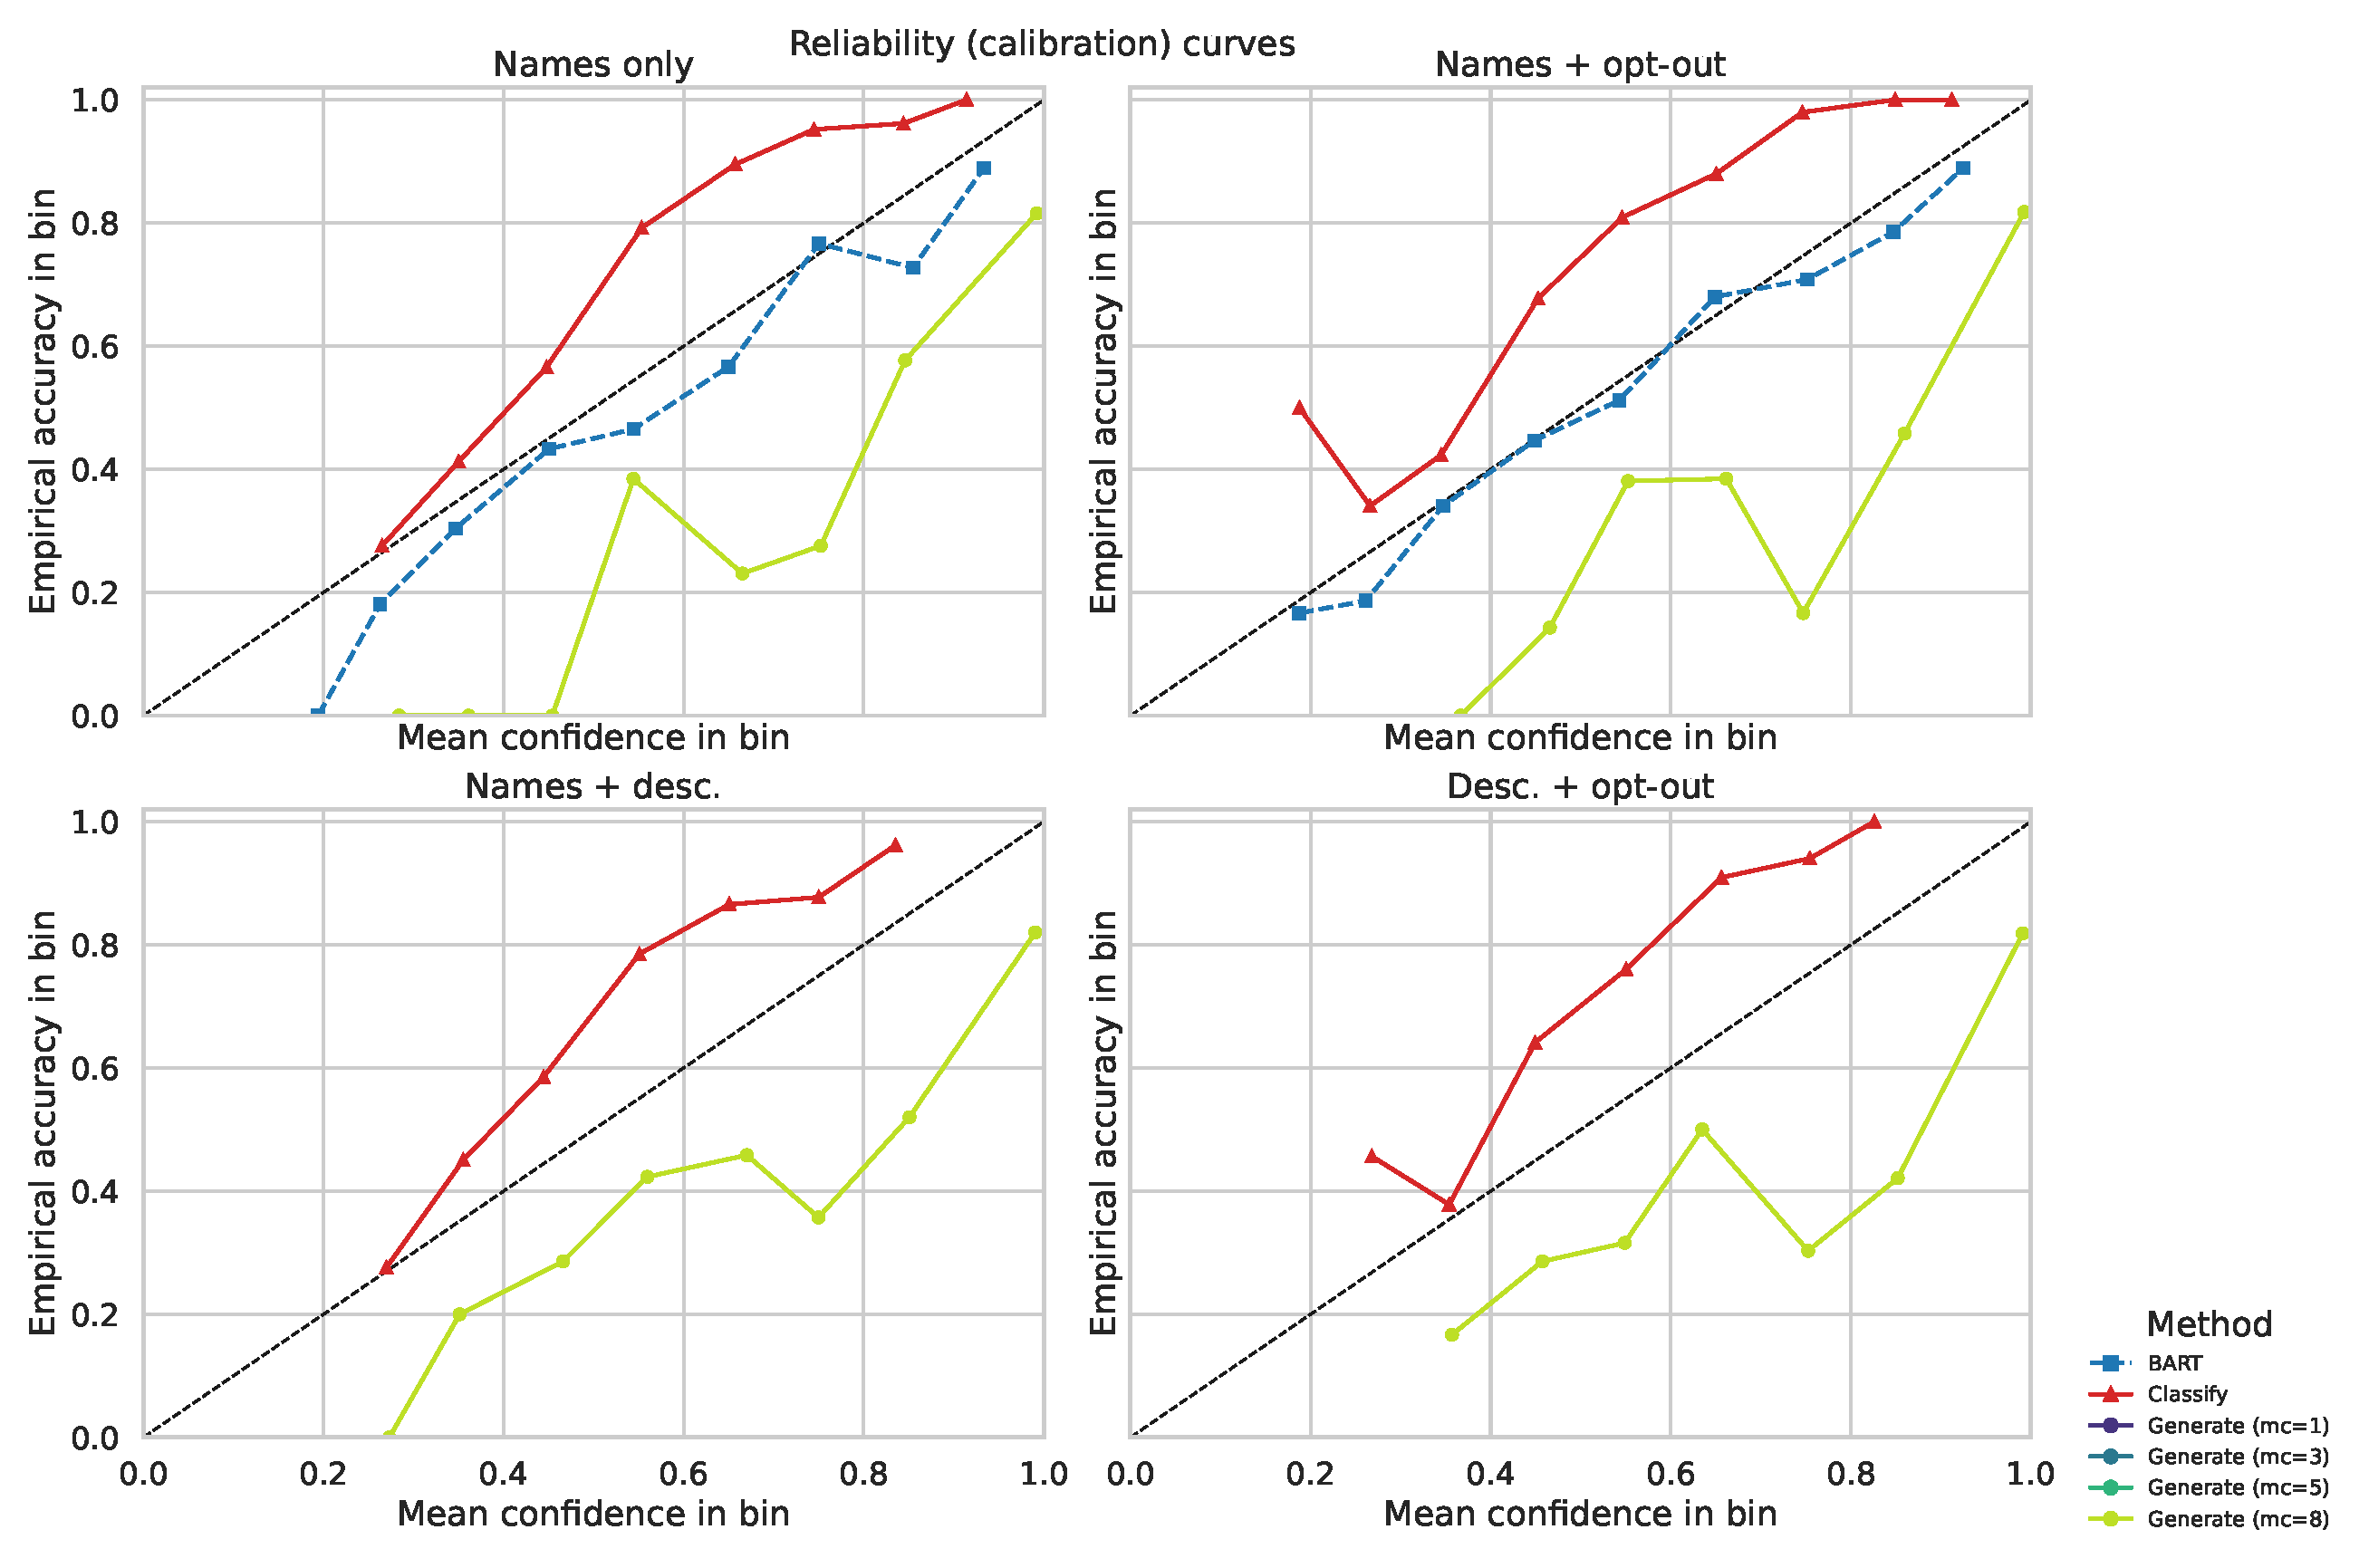
\includegraphics[width=0.95\textwidth]{calibration_curve}
  \caption{Reliability (calibration) curves: empirical accuracy against mean
           confidence within equal-width bins, by choice configuration. The
           dashed diagonal is perfect calibration. BART stays close to the
           diagonal; \texttt{classify} lies \emph{above} it
           (underconfidence---confidence below empirical accuracy), while
           \texttt{generate} lies \emph{below} it (overconfidence---confidence
           above empirical accuracy).}
  \label{fig:calibration}
\end{figure}

\begin{table}[htbp]
  \centering
  \caption{Confidence and calibration across the 10 confidence-bearing
           variations. }
  \label{tab:confidence}
  \resizebox{\textwidth}{!}{%
  \begin{tabular}{lccccccccccc}
    \toprule
    \textbf{Variation} & \textbf{Conf.} & \textbf{Conf.} & $\boldsymbol{r}$
    & \textbf{Gap} & \textbf{Gap} & $\boldsymbol{t}$ & $\boldsymbol{t}$
    & \textbf{ECE} & \textbf{AUC} & \textbf{AUC} & \textbf{Brier} \\
    & (corr.) & (inc.) & & (corr.) & (inc.) & (conf.) & (gap) & & (conf.) & (gap) & \\
    \midrule
    BART (names only) & 0.532 & 0.414 & 0.347 & 0.315 & 0.197 & 8.93 & 6.68 & 0.055 & 0.697 & 0.640 & 0.215 \\
    BART (names + opt-out) & 0.509 & 0.392 & 0.351 & 0.295 & 0.179 & 8.80 & 6.67 & 0.028 & 0.700 & 0.644 & 0.214 \\
    \addlinespace
    Ollama \texttt{classify} (names only) & 0.632 & 0.442 & 0.488 & 0.442 & 0.210 & 14.77 & 14.36 & 0.170 & 0.820 & 0.809 & 0.171 \\
    Ollama \texttt{classify} (names + opt-out) & 0.617 & 0.413 & 0.493 & 0.438 & 0.203 & 15.38 & 14.86 & 0.196 & 0.831 & 0.817 & 0.176 \\
    Ollama \texttt{classify} (names + desc.) & 0.642 & 0.460 & 0.445 & 0.478 & 0.234 & 12.93 & 13.48 & 0.149 & 0.788 & 0.799 & 0.175 \\
    Ollama \texttt{classify} (desc. + opt-out) & 0.627 & 0.425 & 0.484 & 0.475 & 0.206 & 15.30 & 16.07 & 0.177 & 0.821 & 0.831 & 0.174 \\
    \addlinespace
    Ollama \texttt{generate} (names only) & 0.975 & 0.844 & 0.434 & 0.952 & 0.730 & 8.58 & 8.64 & 0.203 & 0.831 & 0.829 & 0.202 \\
    Ollama \texttt{generate} (names + opt-out) & 0.977 & 0.849 & 0.426 & 0.957 & 0.741 & 7.98 & 8.01 & 0.202 & 0.818 & 0.816 & 0.200 \\
    Ollama \texttt{generate} (names + desc.) & 0.955 & 0.831 & 0.378 & 0.921 & 0.716 & 8.10 & 8.08 & 0.193 & 0.783 & 0.782 & 0.207 \\
    Ollama \texttt{generate} (desc. + opt-out) & 0.961 & 0.823 & 0.420 & 0.933 & 0.703 & 8.92 & 9.00 & 0.205 & 0.822 & 0.821 & 0.210 \\
    \bottomrule
  \end{tabular}}
  \footnotesize{
    ``Conf'' is the mean predicted-label confidence on
    correct/incorrect predictions; ``Gap'' is the mean score gap
    (top minus second probability); $r$ is the point-biserial
    correlation between confidence and correctness; $t$ is the
    one-tailed Welch statistic (correct $>$ incorrect) for each
    metric (all $p<0.001$ after BH correction). ECE uses 10
    equal-width bins; AUC is the ROC-AUC of each score against
    correctness; Brier is the mean squared error of confidence.
    scikit-llm is omitted (label-only). For \texttt{generate} only
     the default single-call setting is reported (larger budgets are
     identical on this task).
  }
\end{table}

\paragraph{Threshold-based discrimination.}
A practitioner does not need well-calibrated probabilities to deploy triage:
it suffices that a threshold on confidence, or on the score gap, separates
correct from incorrect predictions. The distributional basis for this
separation is visible in the confidence and score-gap boxplots
(Figures~\ref{fig:conf-boxplots} and \ref{fig:gap-boxplots}): across all 10
confidence-bearing variations, correct predictions consistently concentrate at
higher values than incorrect ones. Table~\ref{tab:threshold} reports, for the
six headline variations, the ROC-AUC of each score and the Youden-optimal
threshold ($J=\text{TPR}-\text{FPR}$, true positive rate minus false
positive rate) with the resulting selective accuracy
(accuracy among items above the threshold) and coverage. For
\texttt{classify}, both scores discriminate strongly: AUC is 0.79--0.83
whether one ranks by confidence or by the score gap, and abstaining below the
Youden-optimal margin threshold lifts accuracy from a 71--75\% baseline to
89--93\% while retaining 55--66\% of the items (e.g., names only: 75.5\%
$\to$ 92.8\% at 58.6\% coverage). The score gap is as informative as
confidence and sometimes more so (desc.\ + opt-out: AUC 0.831 vs.\ 0.821).
BART discriminates more weakly (AUC $\approx$ 0.70), and its optimal margin
threshold is aggressive (coverage $\approx$ 27--33\%). The selective-accuracy
and coverage curves in Figures~\ref{fig:tradeoff} and \ref{fig:tradeoff-margin}
show the same effect continuously: for both ranking variables, accuracy rises
as the threshold tightens, and the margin offers a second, complementary
operating axis. This validates threshold-based triage for \texttt{classify}
with either score, and quantifies the accuracy--coverage trade-off that
distinguishes \texttt{ollama-classifier} from the label-only scikit-llm.

\begin{table}[htbp]
  \centering
  \caption{Threshold discrimination for the six headline variations.}
  \label{tab:threshold}
  \resizebox{\textwidth}{!}{%
  \begin{tabular}{lcccccccc}
    \toprule
    & \multicolumn{4}{c}{\textbf{Confidence threshold}}
    & \multicolumn{4}{c}{\textbf{Margin (score-gap) threshold}} \\
    \cmidrule(lr){2-5}\cmidrule(lr){6-9}
    \textbf{Variation} & \textbf{AUC} & \textbf{thr.} & \textbf{sel.\ acc.}
    & \textbf{cov.} & \textbf{AUC} & \textbf{thr.} & \textbf{sel.\ acc.}
    & \textbf{cov.} \\
    & & & (\%) & (\%) & & & (\%) & (\%) \\
    \midrule
    BART (names only) & 0.697 & 0.42 & 54.4 & 53.4 & 0.640 & 0.34 & 60.9 & 27.3 \\
    BART (names + opt-out) & 0.700 & 0.41 & 56.3 & 51.8 & 0.644 & 0.27 & 59.5 & 33.3 \\
    \addlinespace
    Ollama \texttt{classify} (names only) & 0.820 & 0.52 & 91.3 & 64.7 & 0.809 & 0.36 & 92.8 & 58.6 \\
    Ollama \texttt{classify} (names + opt-out) & 0.831 & 0.53 & 92.4 & 59.3 & 0.817 & 0.34 & 93.0 & 60.0 \\
    Ollama \texttt{classify} (names + desc.) & 0.788 & 0.54 & 89.0 & 61.2 & 0.799 & 0.30 & 89.0 & 65.6 \\
    Ollama \texttt{classify} (desc. + opt-out) & 0.821 & 0.55 & 93.4 & 55.0 & 0.831 & 0.32 & 91.8 & 62.6 \\
    \bottomrule
  \end{tabular}}
  \footnotesize{
    AUC is the ROC-AUC of each score against correctness; the remaining
    columns report the Youden-optimal threshold ($J=\text{TPR}-\text{FPR}$)
    and the selective accuracy (accuracy among items with score
    $\geq$ threshold) and coverage (\% retained) at that threshold, for
    confidence and for the score gap (margin) separately.
}
\end{table}

\begin{figure}[htbp]
  \centering
  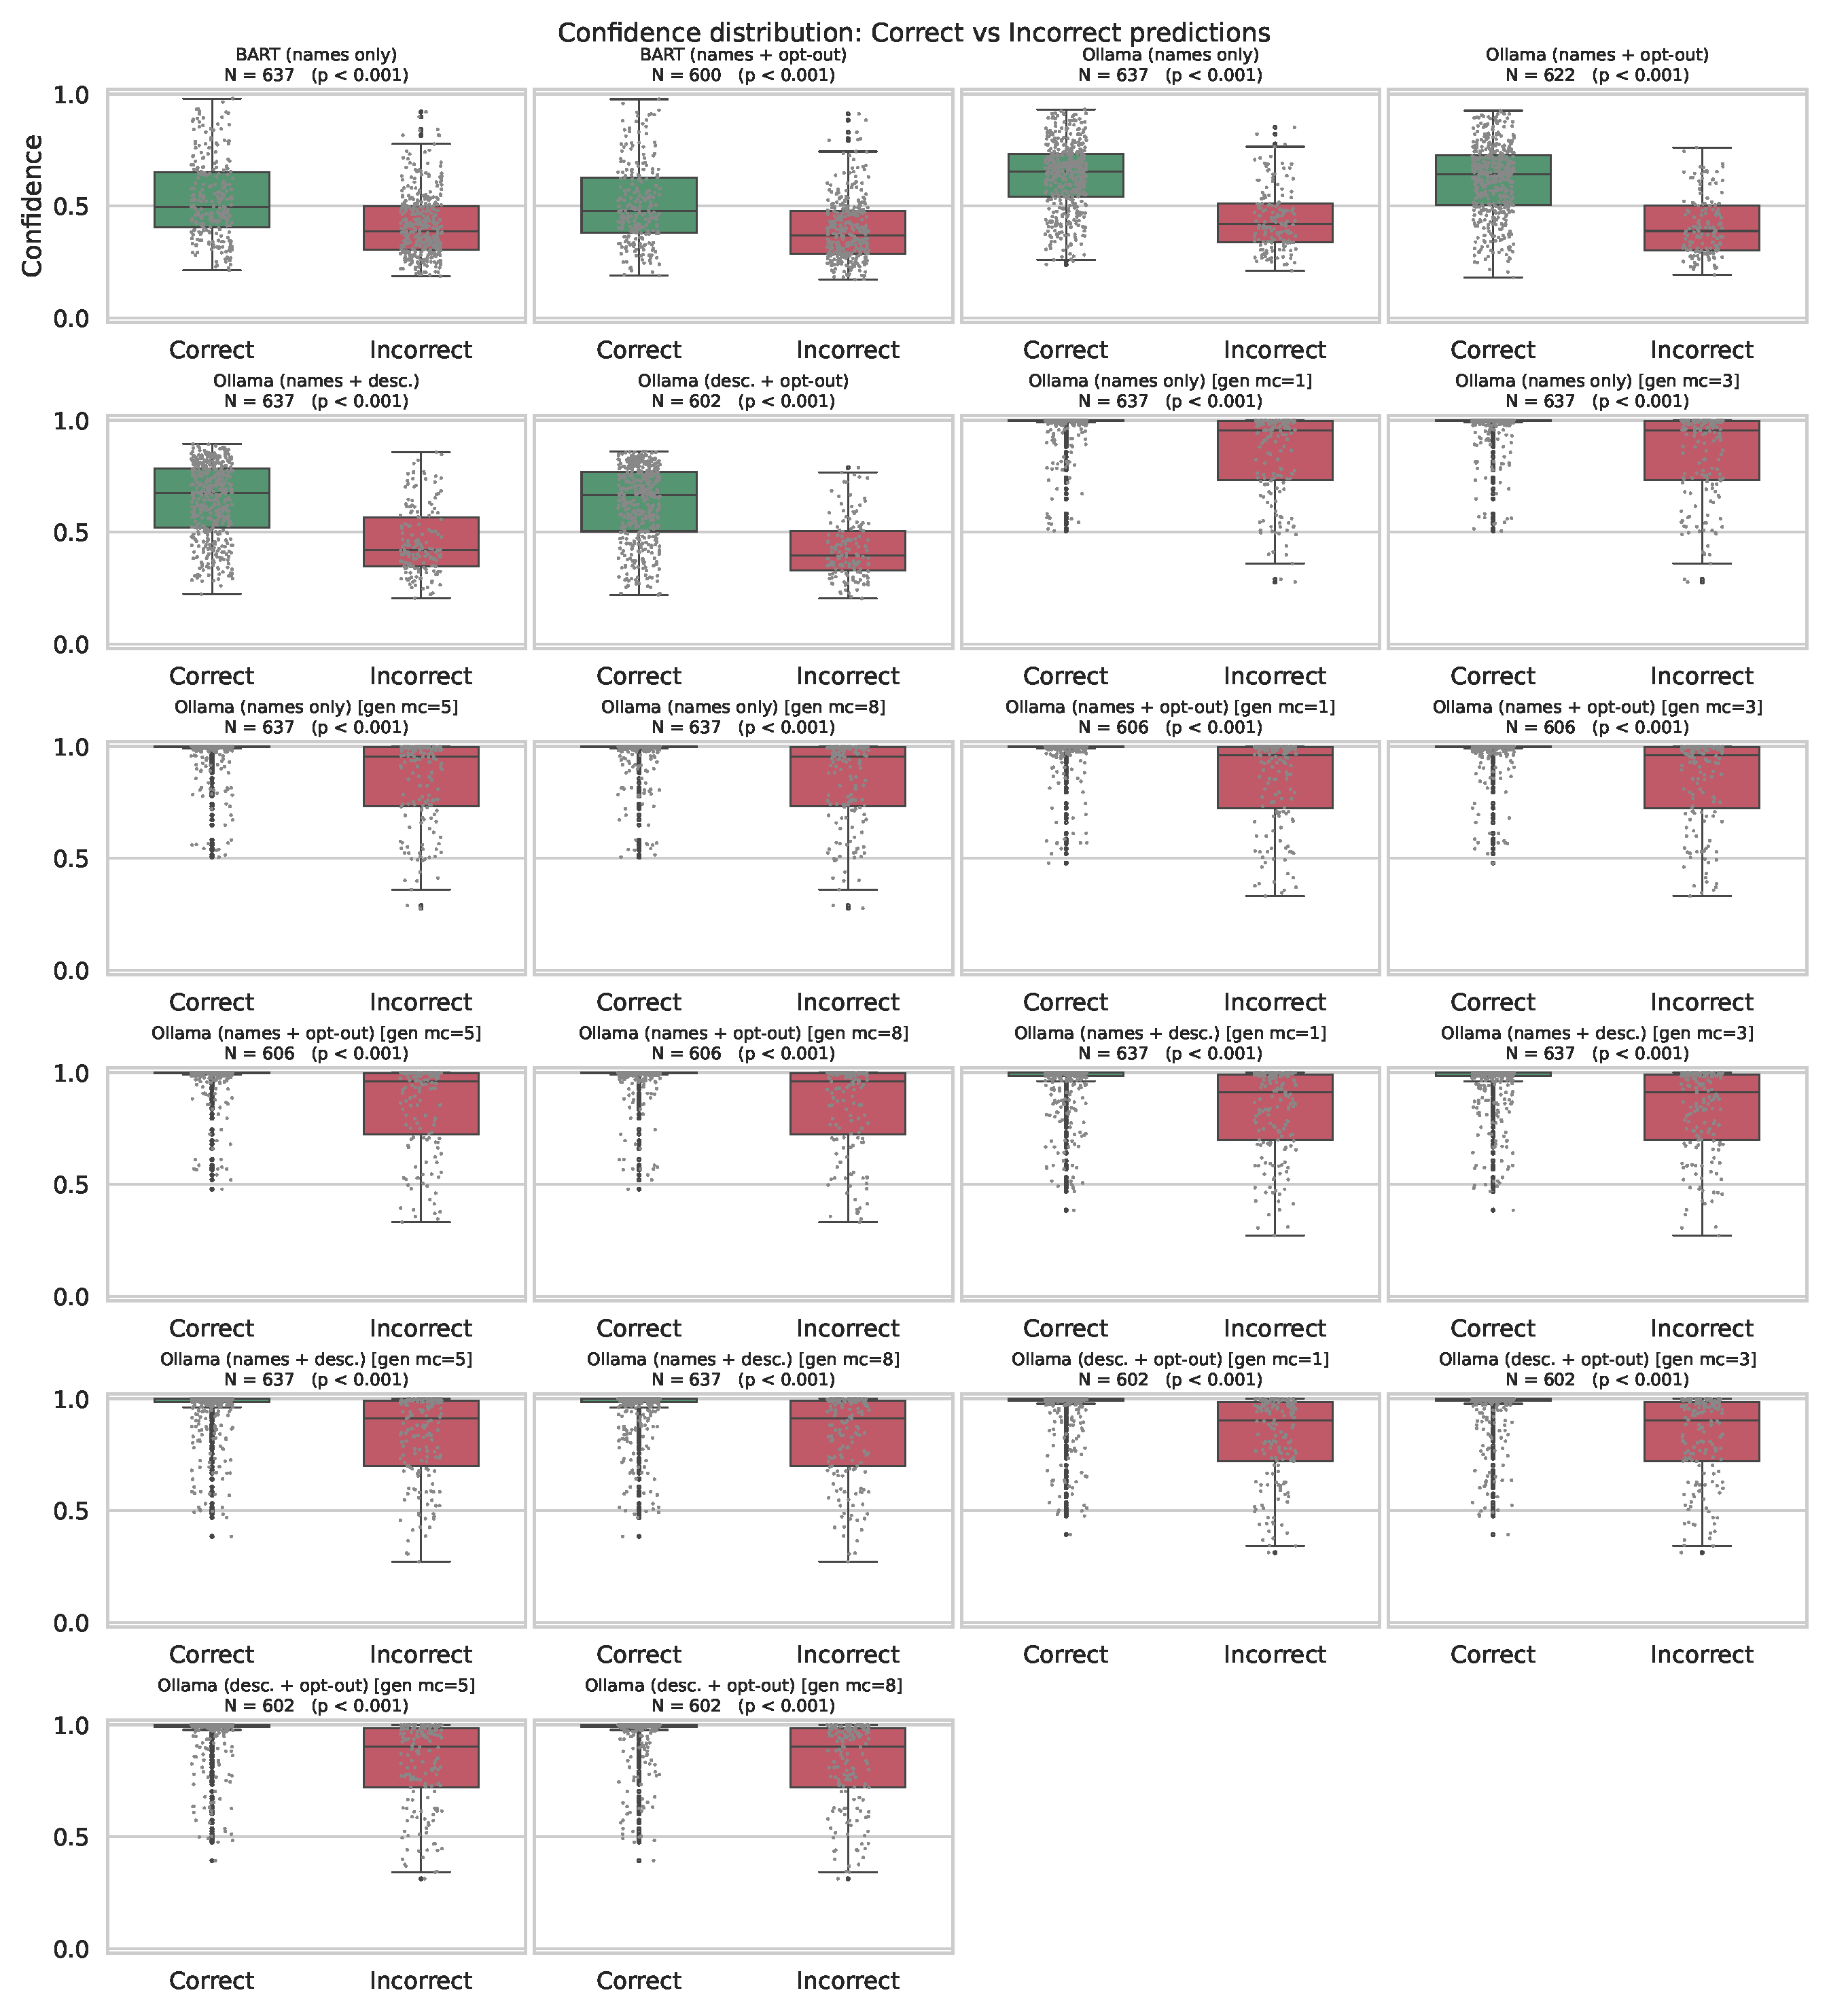
\includegraphics[width=0.95\textwidth]{confidence_boxplots}
   \caption{Confidence distributions for correct (green) and incorrect (red)
            predictions across all 10 confidence-bearing variations. Each panel
           shows the boxplot and individual data points (jittered) for one
           variation, annotated with the sample size $N$ and the one-tailed
           Welch $t$-test $p$-value (correct $>$ incorrect). Correct
           predictions consistently concentrate at higher confidence than
           incorrect ones.}
  \label{fig:conf-boxplots}
\end{figure}

\begin{figure}[htbp]
  \centering
  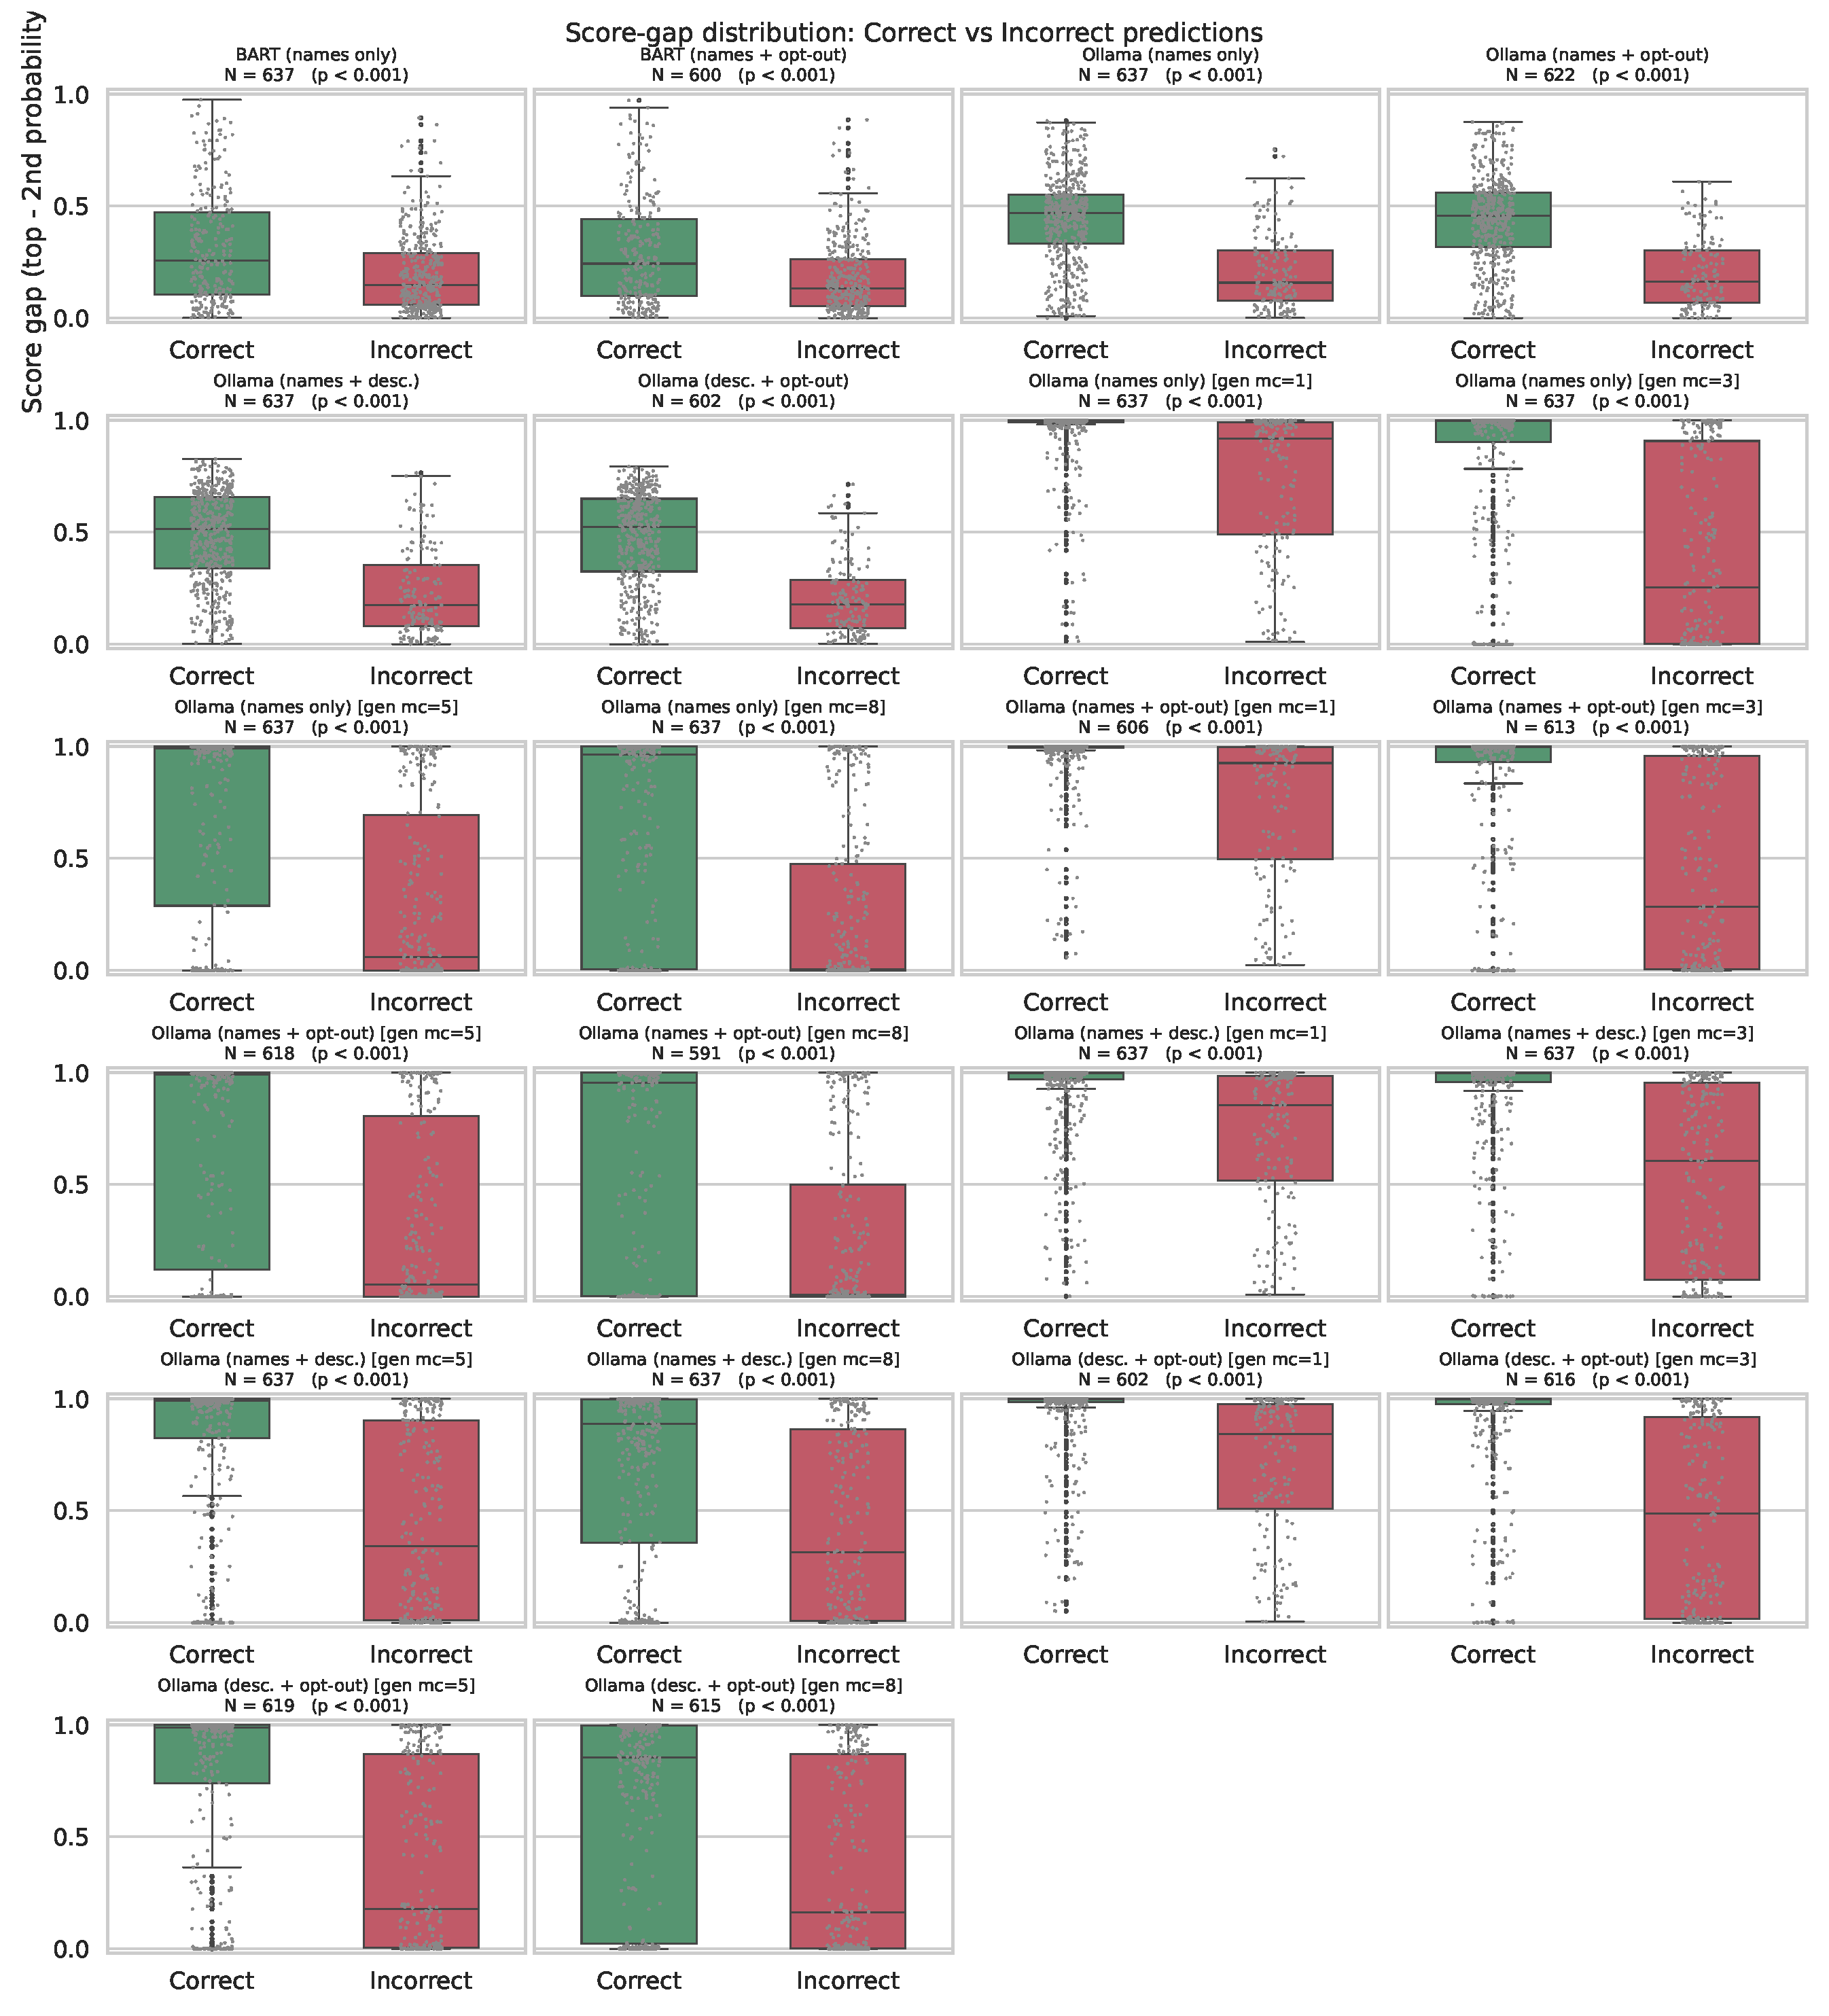
\includegraphics[width=0.95\textwidth]{scoregap_boxplots}
   \caption{Score-gap (top minus second-highest class probability)
            distributions for correct and incorrect predictions across all 10
            confidence-bearing variations. Same layout as
           Figure~\ref{fig:conf-boxplots}. The score gap discriminates
           correctness comparably to confidence, with correct predictions
           showing larger margins.}
  \label{fig:gap-boxplots}
\end{figure}

\begin{figure}[htbp]
  \centering
  \begin{subfigure}{0.49\textwidth}
    \centering
    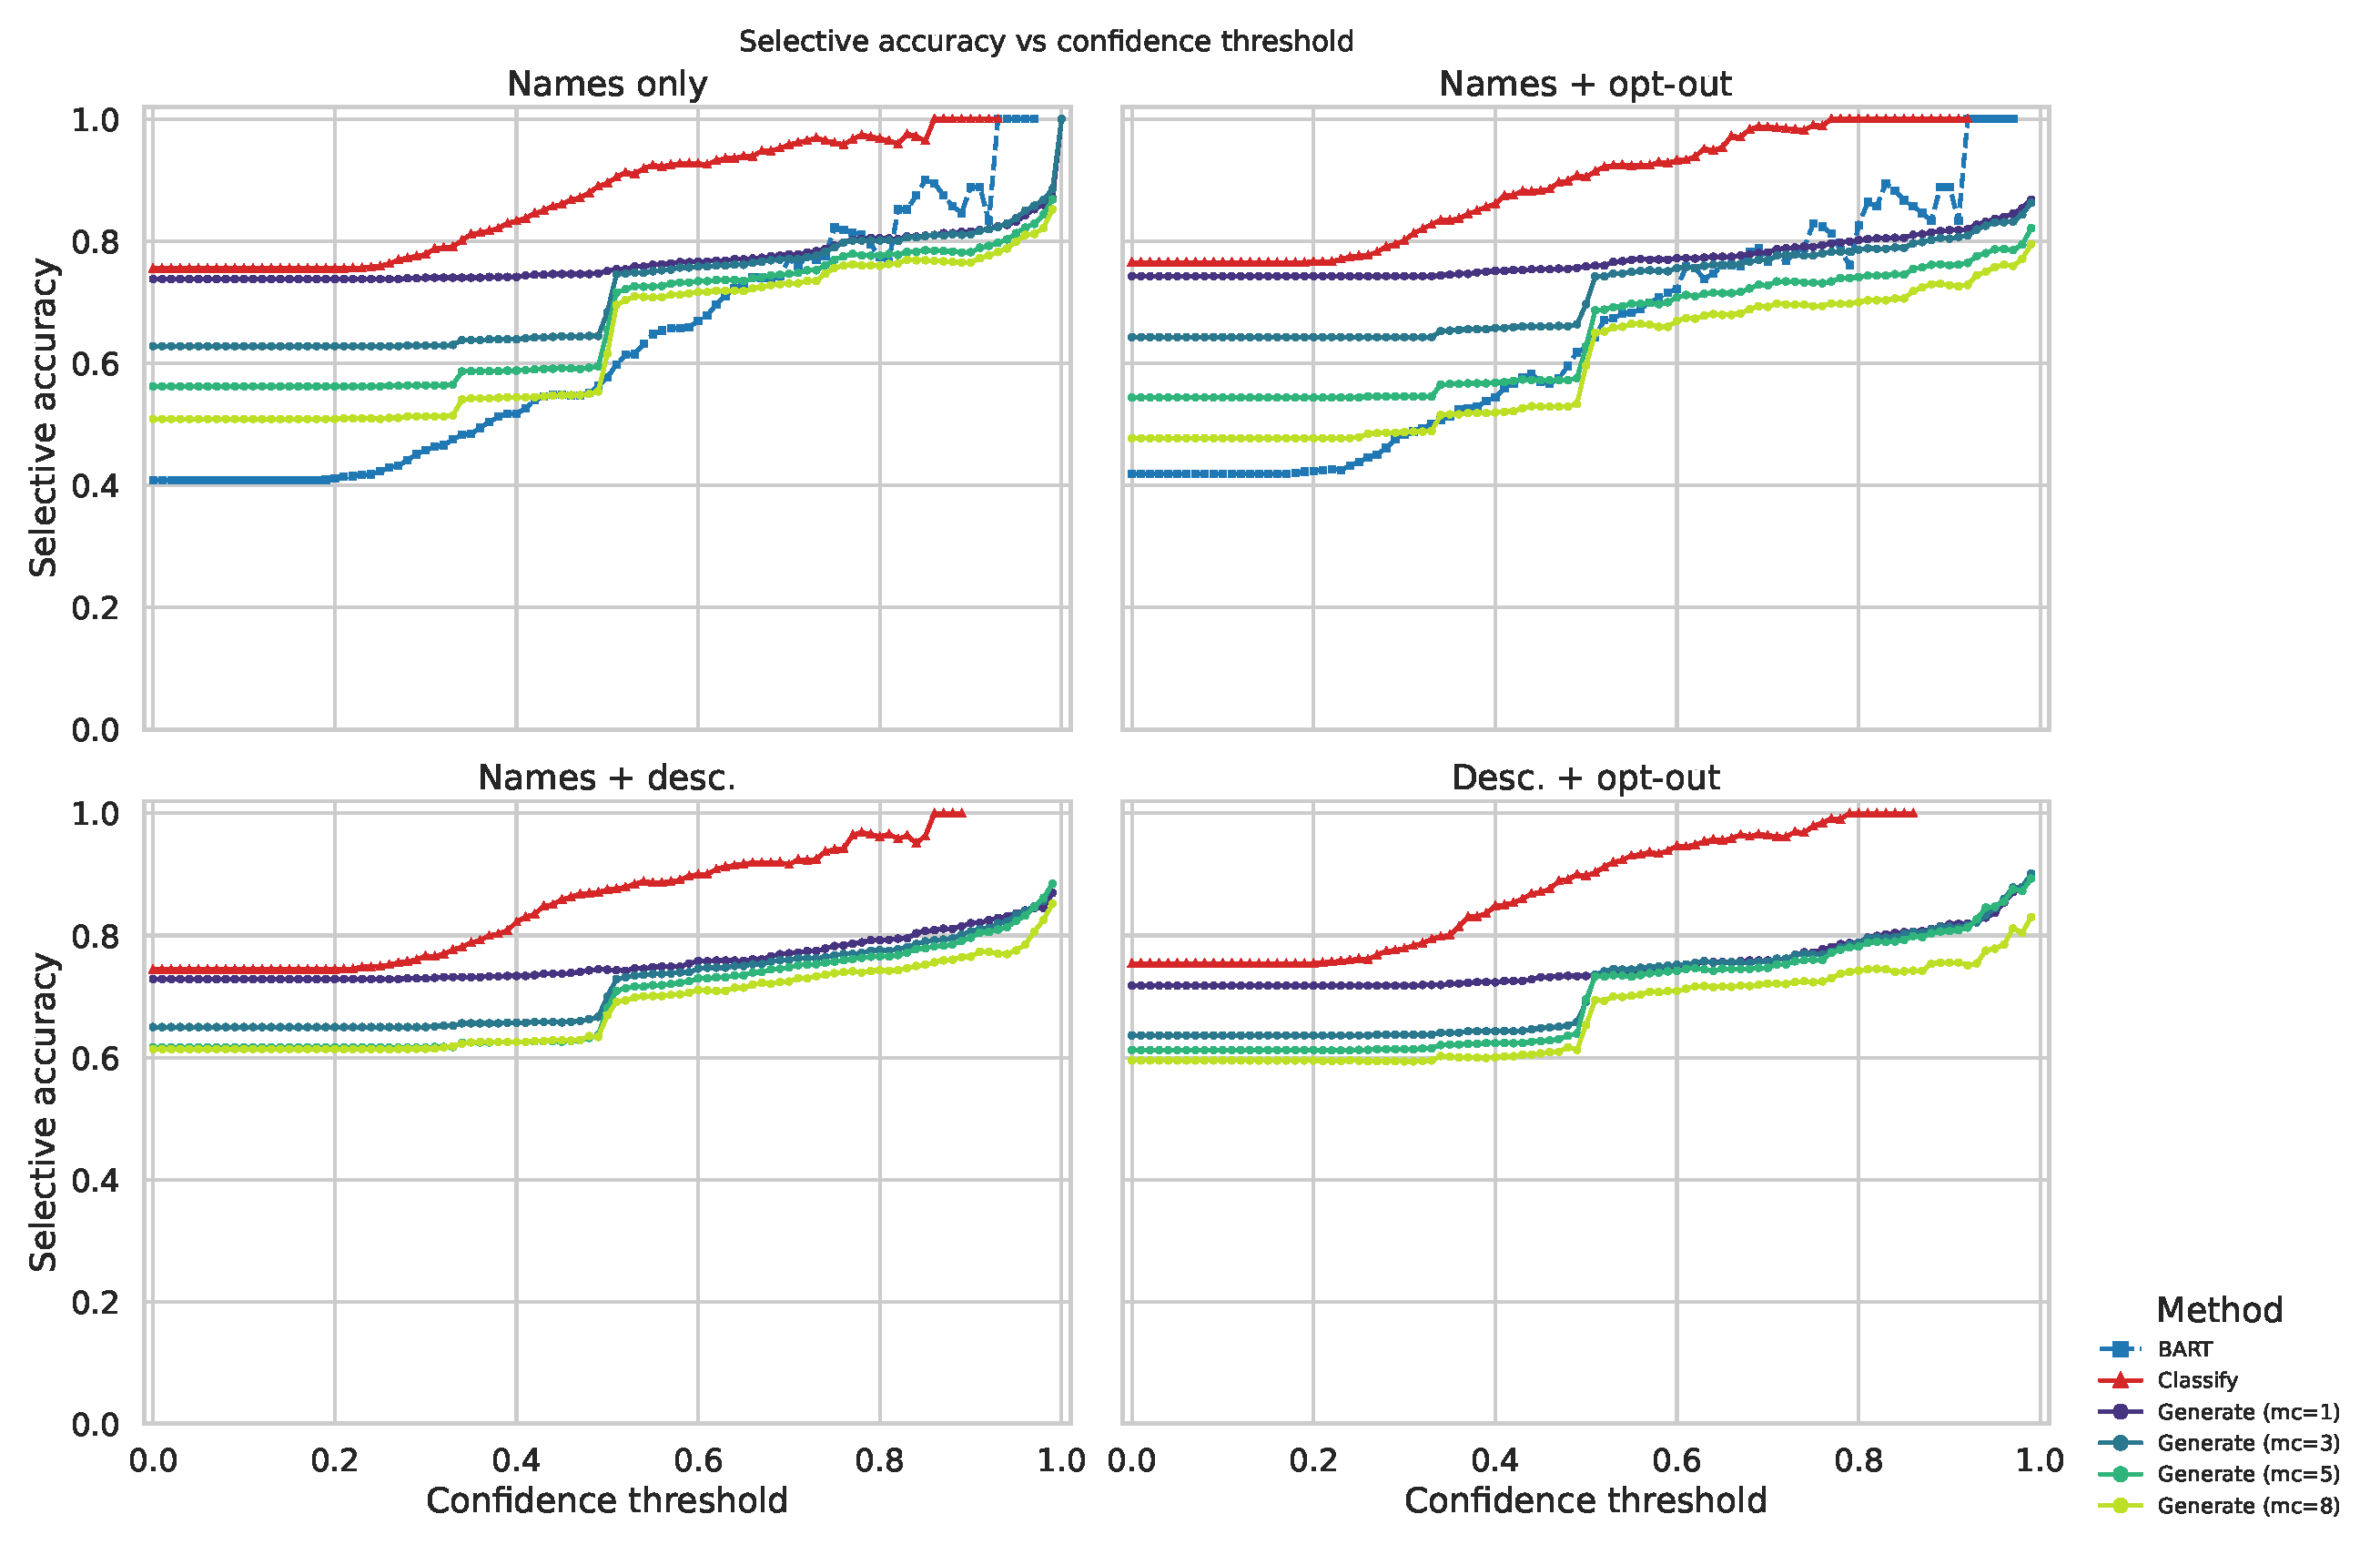
\includegraphics[width=\textwidth]{selective_accuracy}
    \caption{Selective accuracy vs.\ confidence threshold.}
    \label{fig:selective-accuracy}
  \end{subfigure}
  \hfill
  \begin{subfigure}{0.49\textwidth}
    \centering
    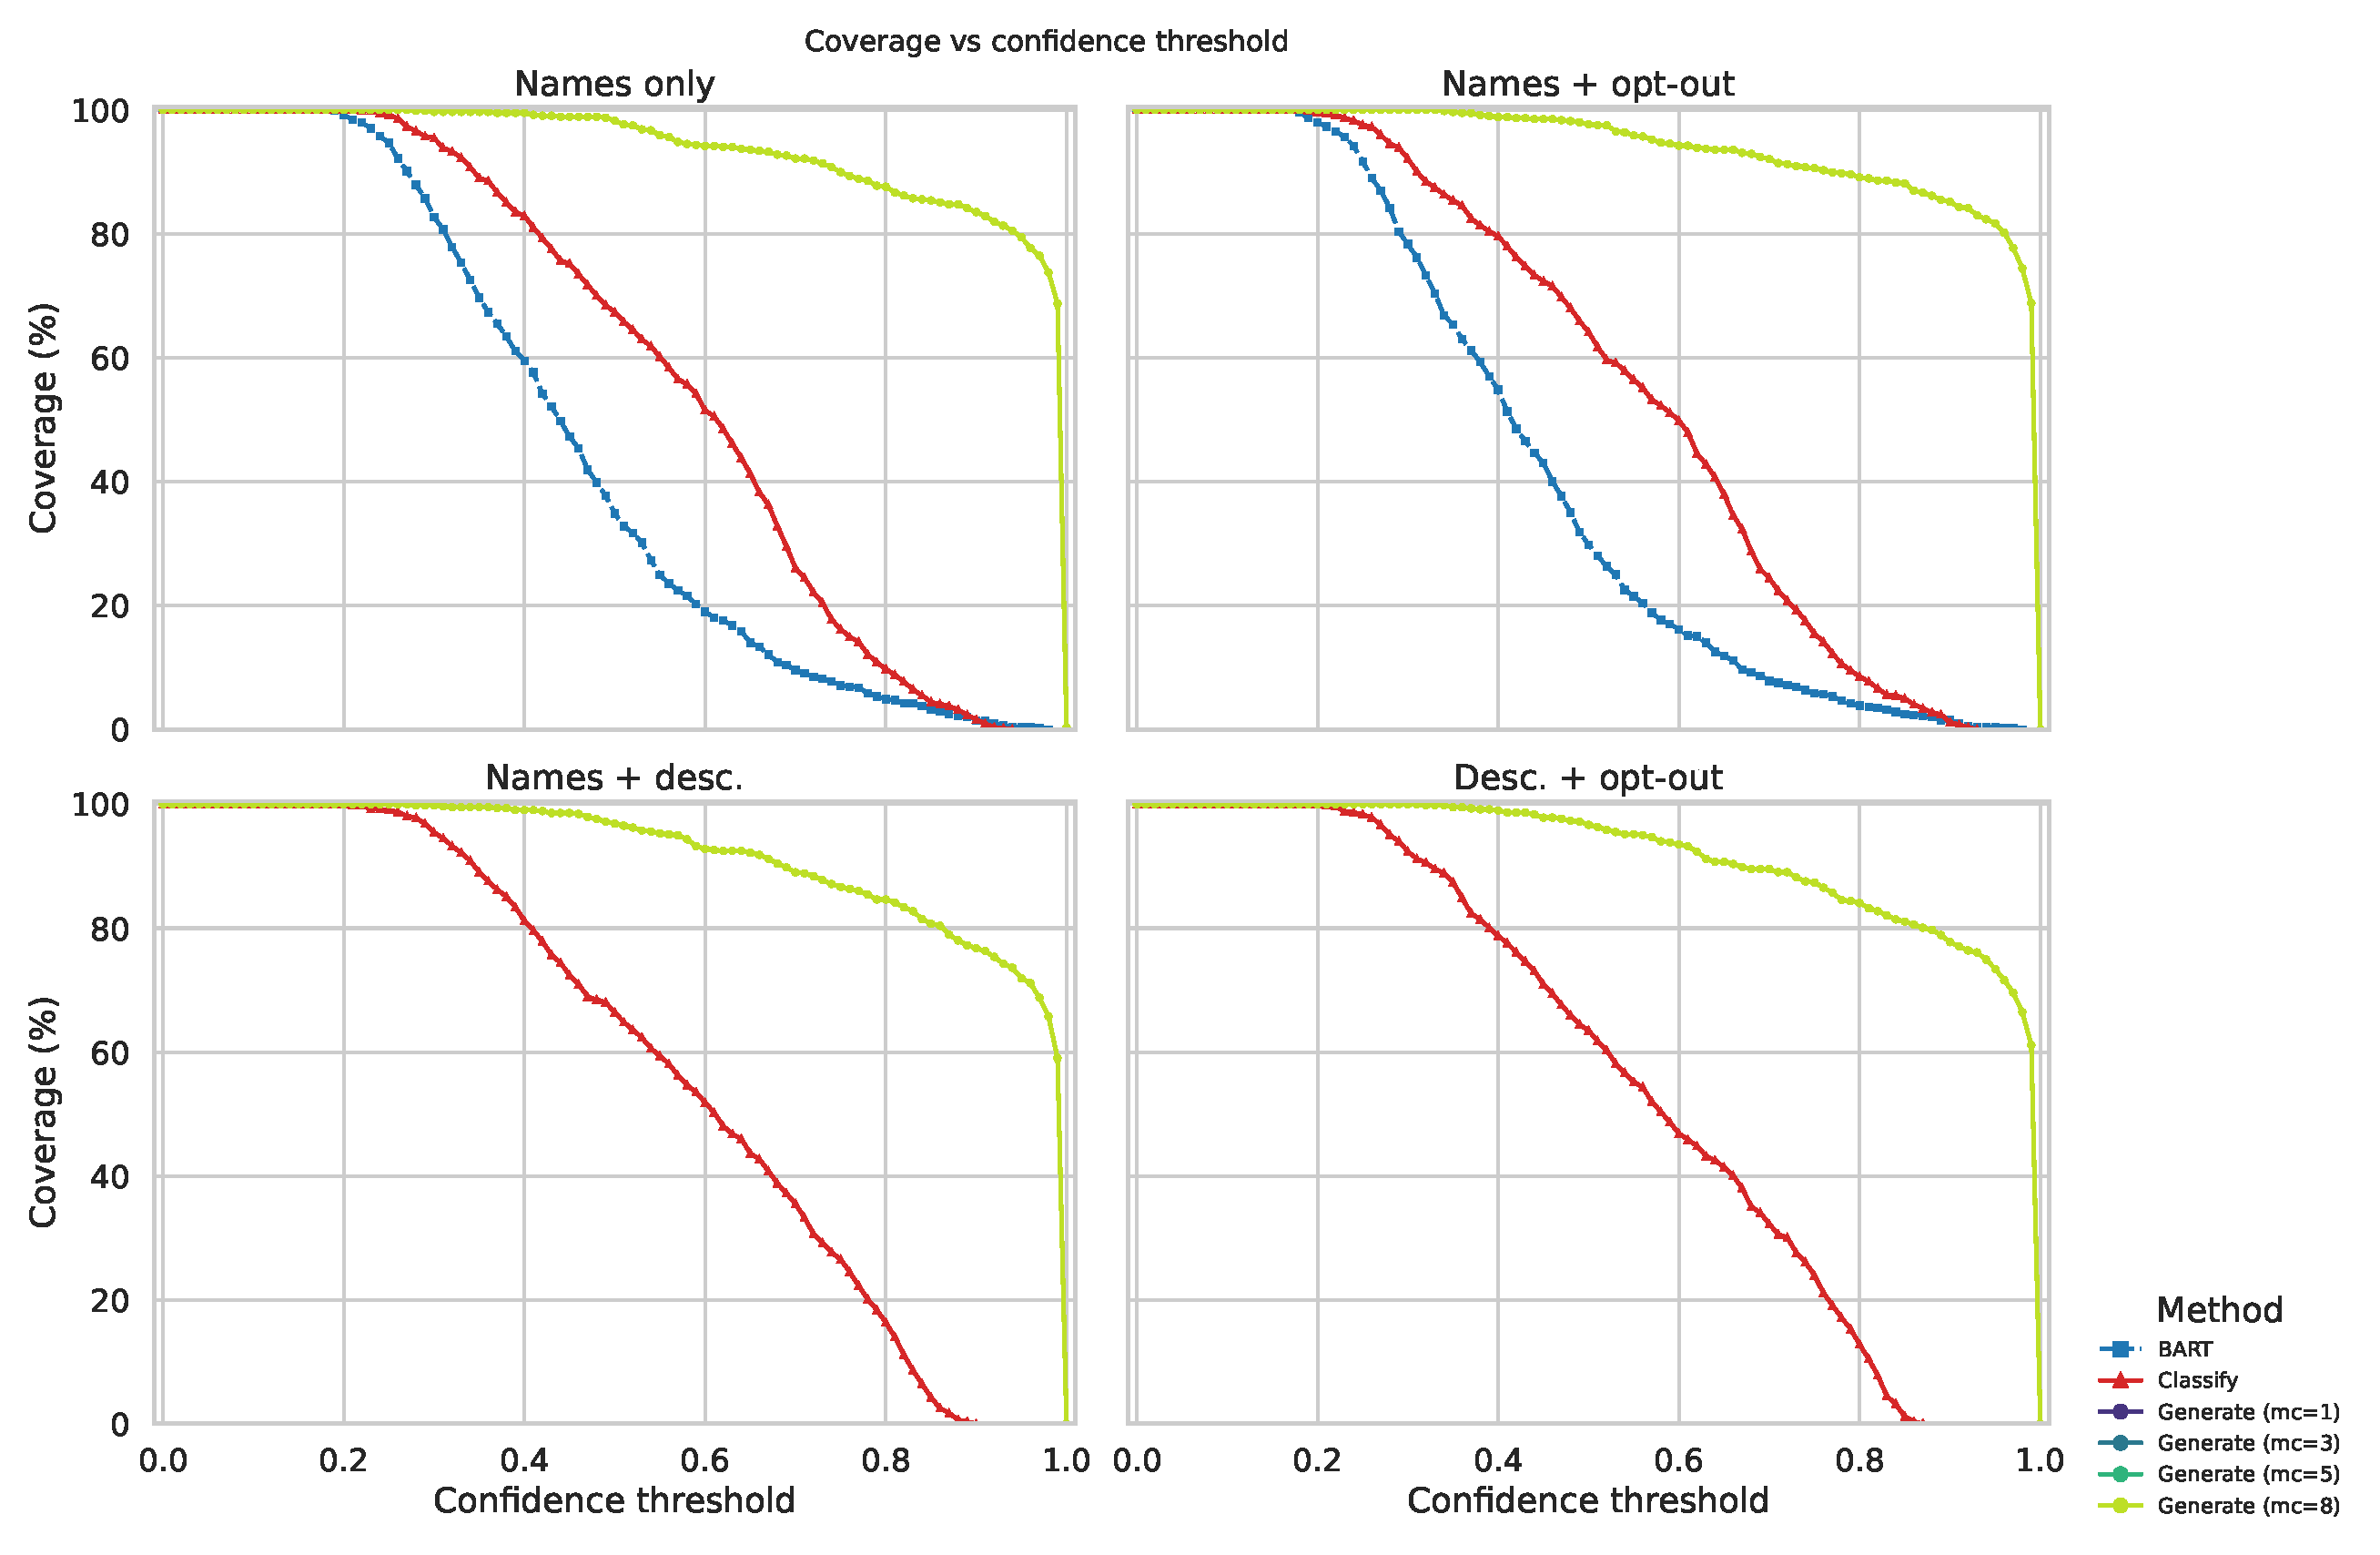
\includegraphics[width=\textwidth]{coverage_curve}
    \caption{Coverage vs.\ confidence threshold.}
    \label{fig:coverage}
  \end{subfigure}
  \caption{Accuracy--coverage trade-off under thresholding on the predicted-label
           confidence, by choice configuration. BART offers a smoother trade-off;
           the generative methods gain selective accuracy quickly because their
           confidence is concentrated high.}
  \label{fig:tradeoff}
\end{figure}

\begin{figure}[htbp]
  \centering
  \begin{subfigure}{0.49\textwidth}
    \centering
    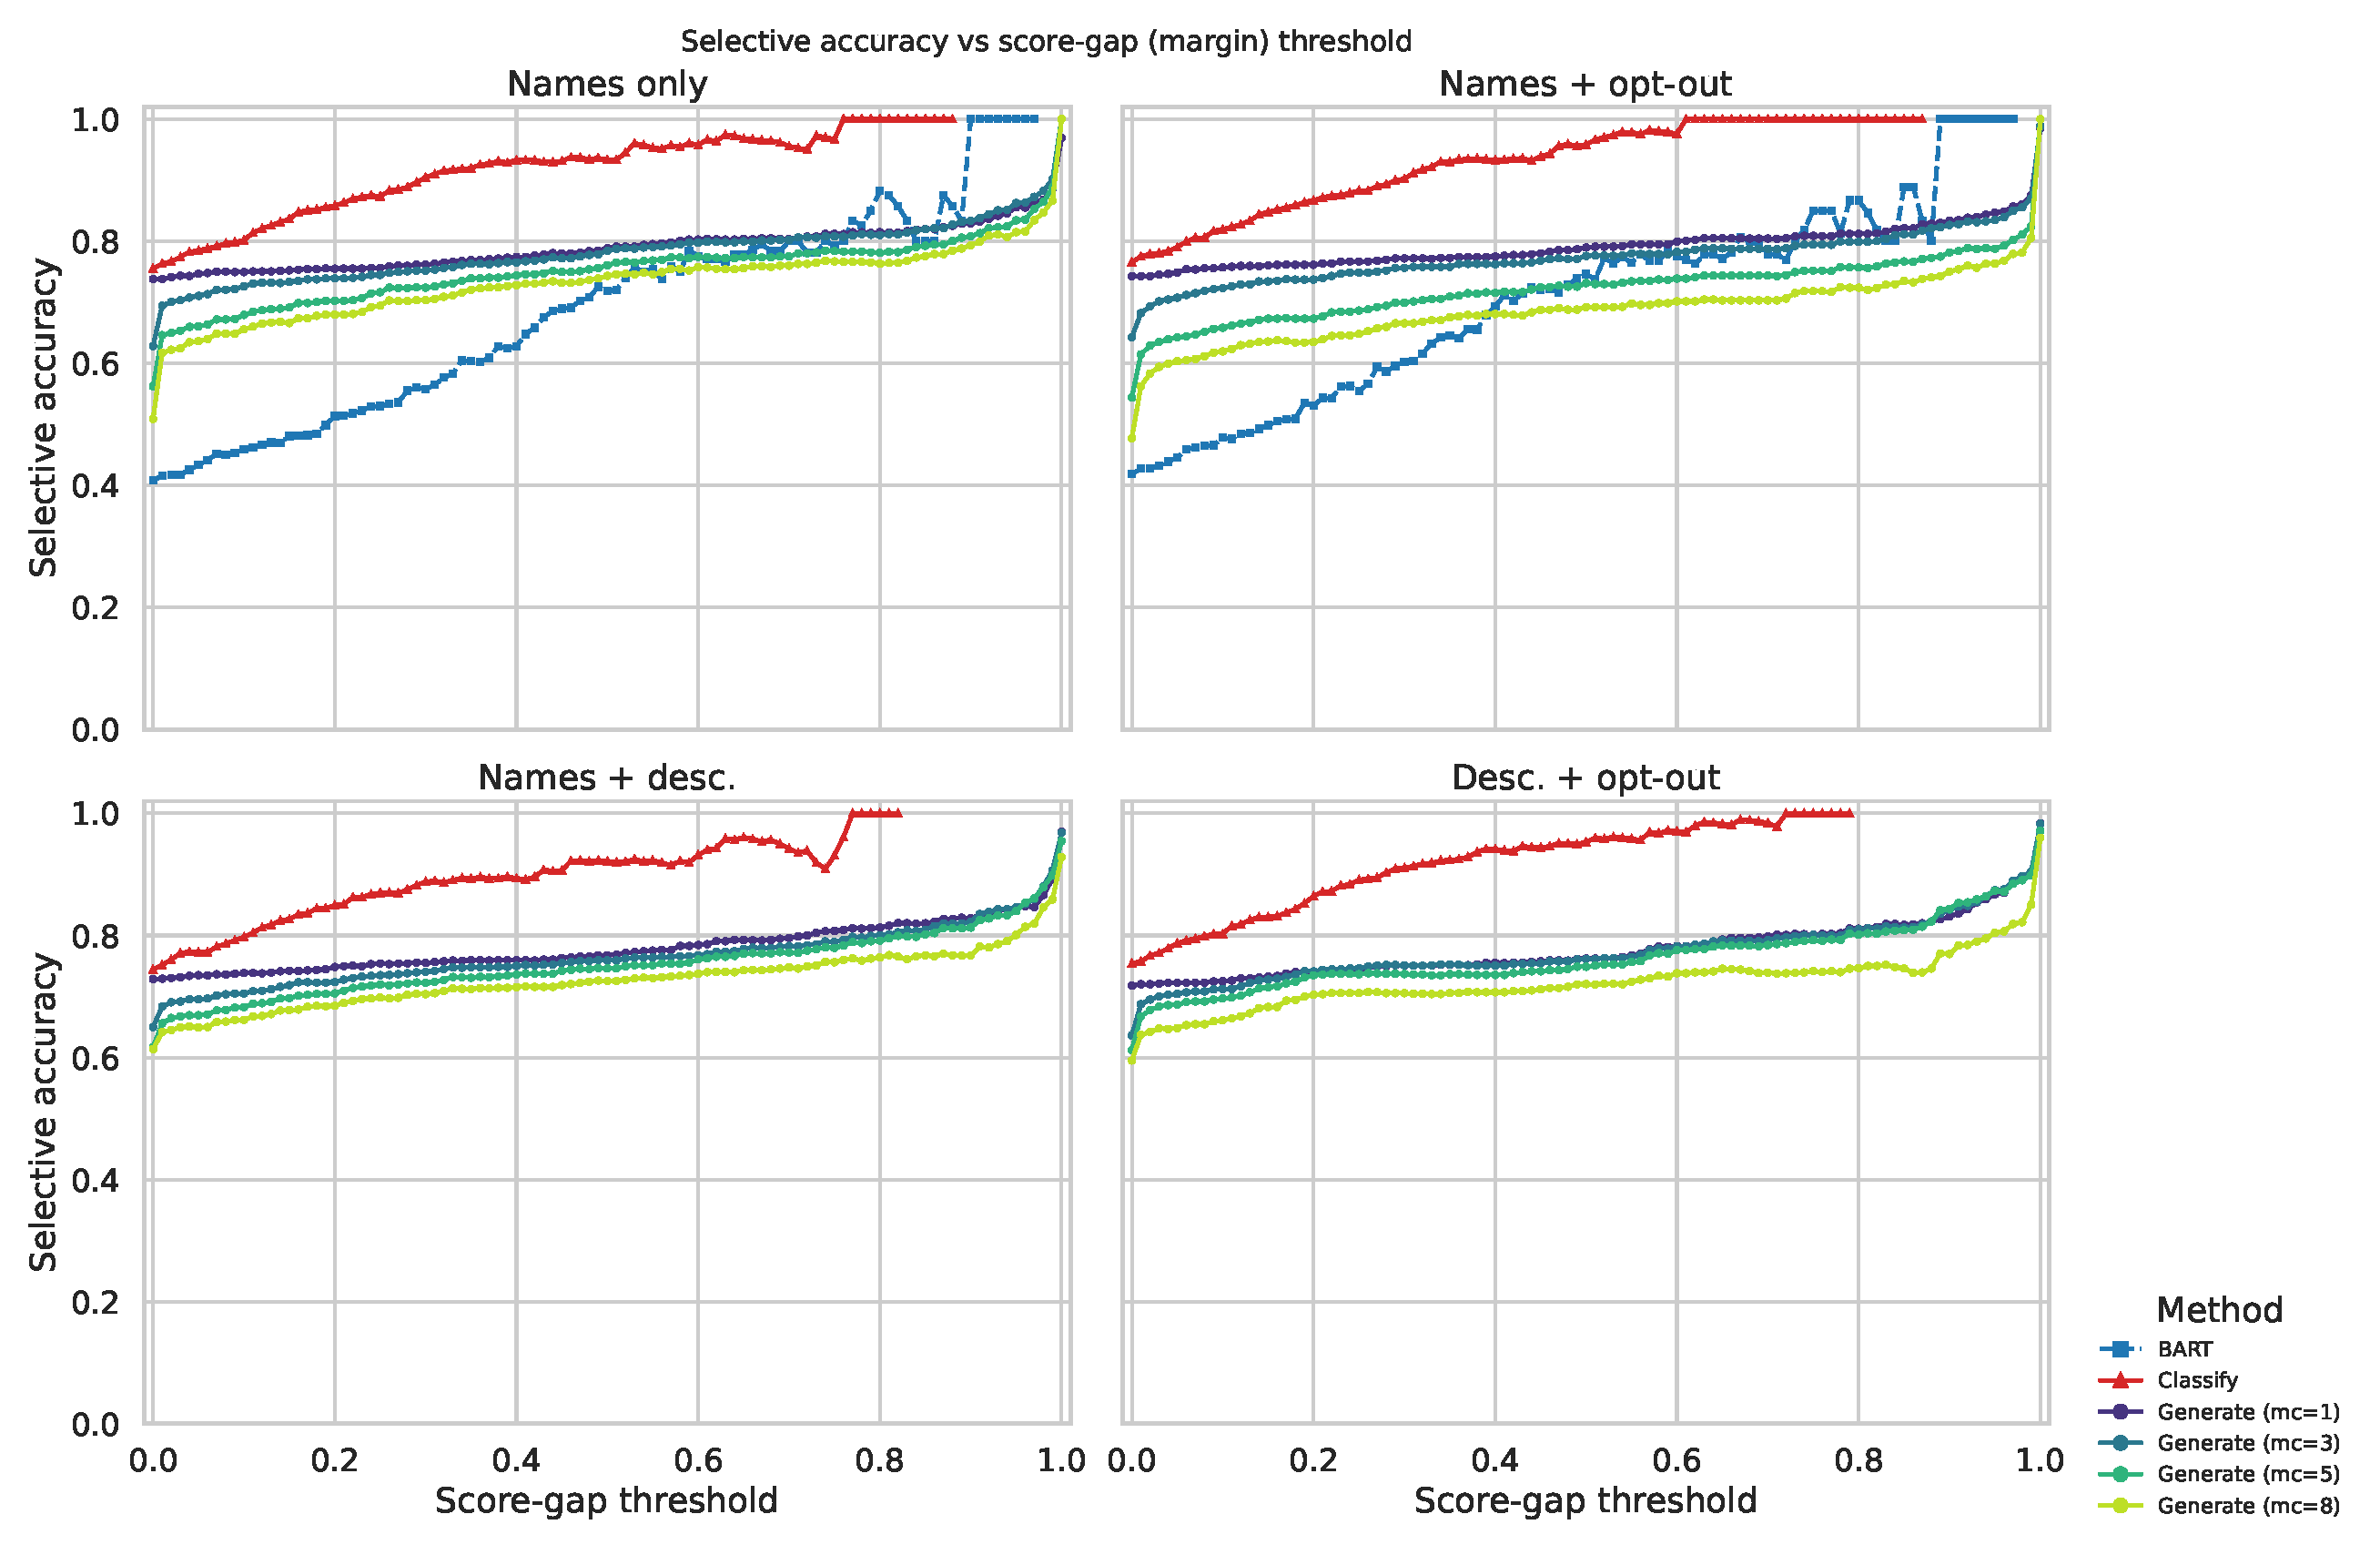
\includegraphics[width=\textwidth]{selective_accuracy_margin}
    \caption{Selective accuracy vs.\ score-gap threshold.}
    \label{fig:selective-accuracy-margin}
  \end{subfigure}
  \hfill
  \begin{subfigure}{0.49\textwidth}
    \centering
    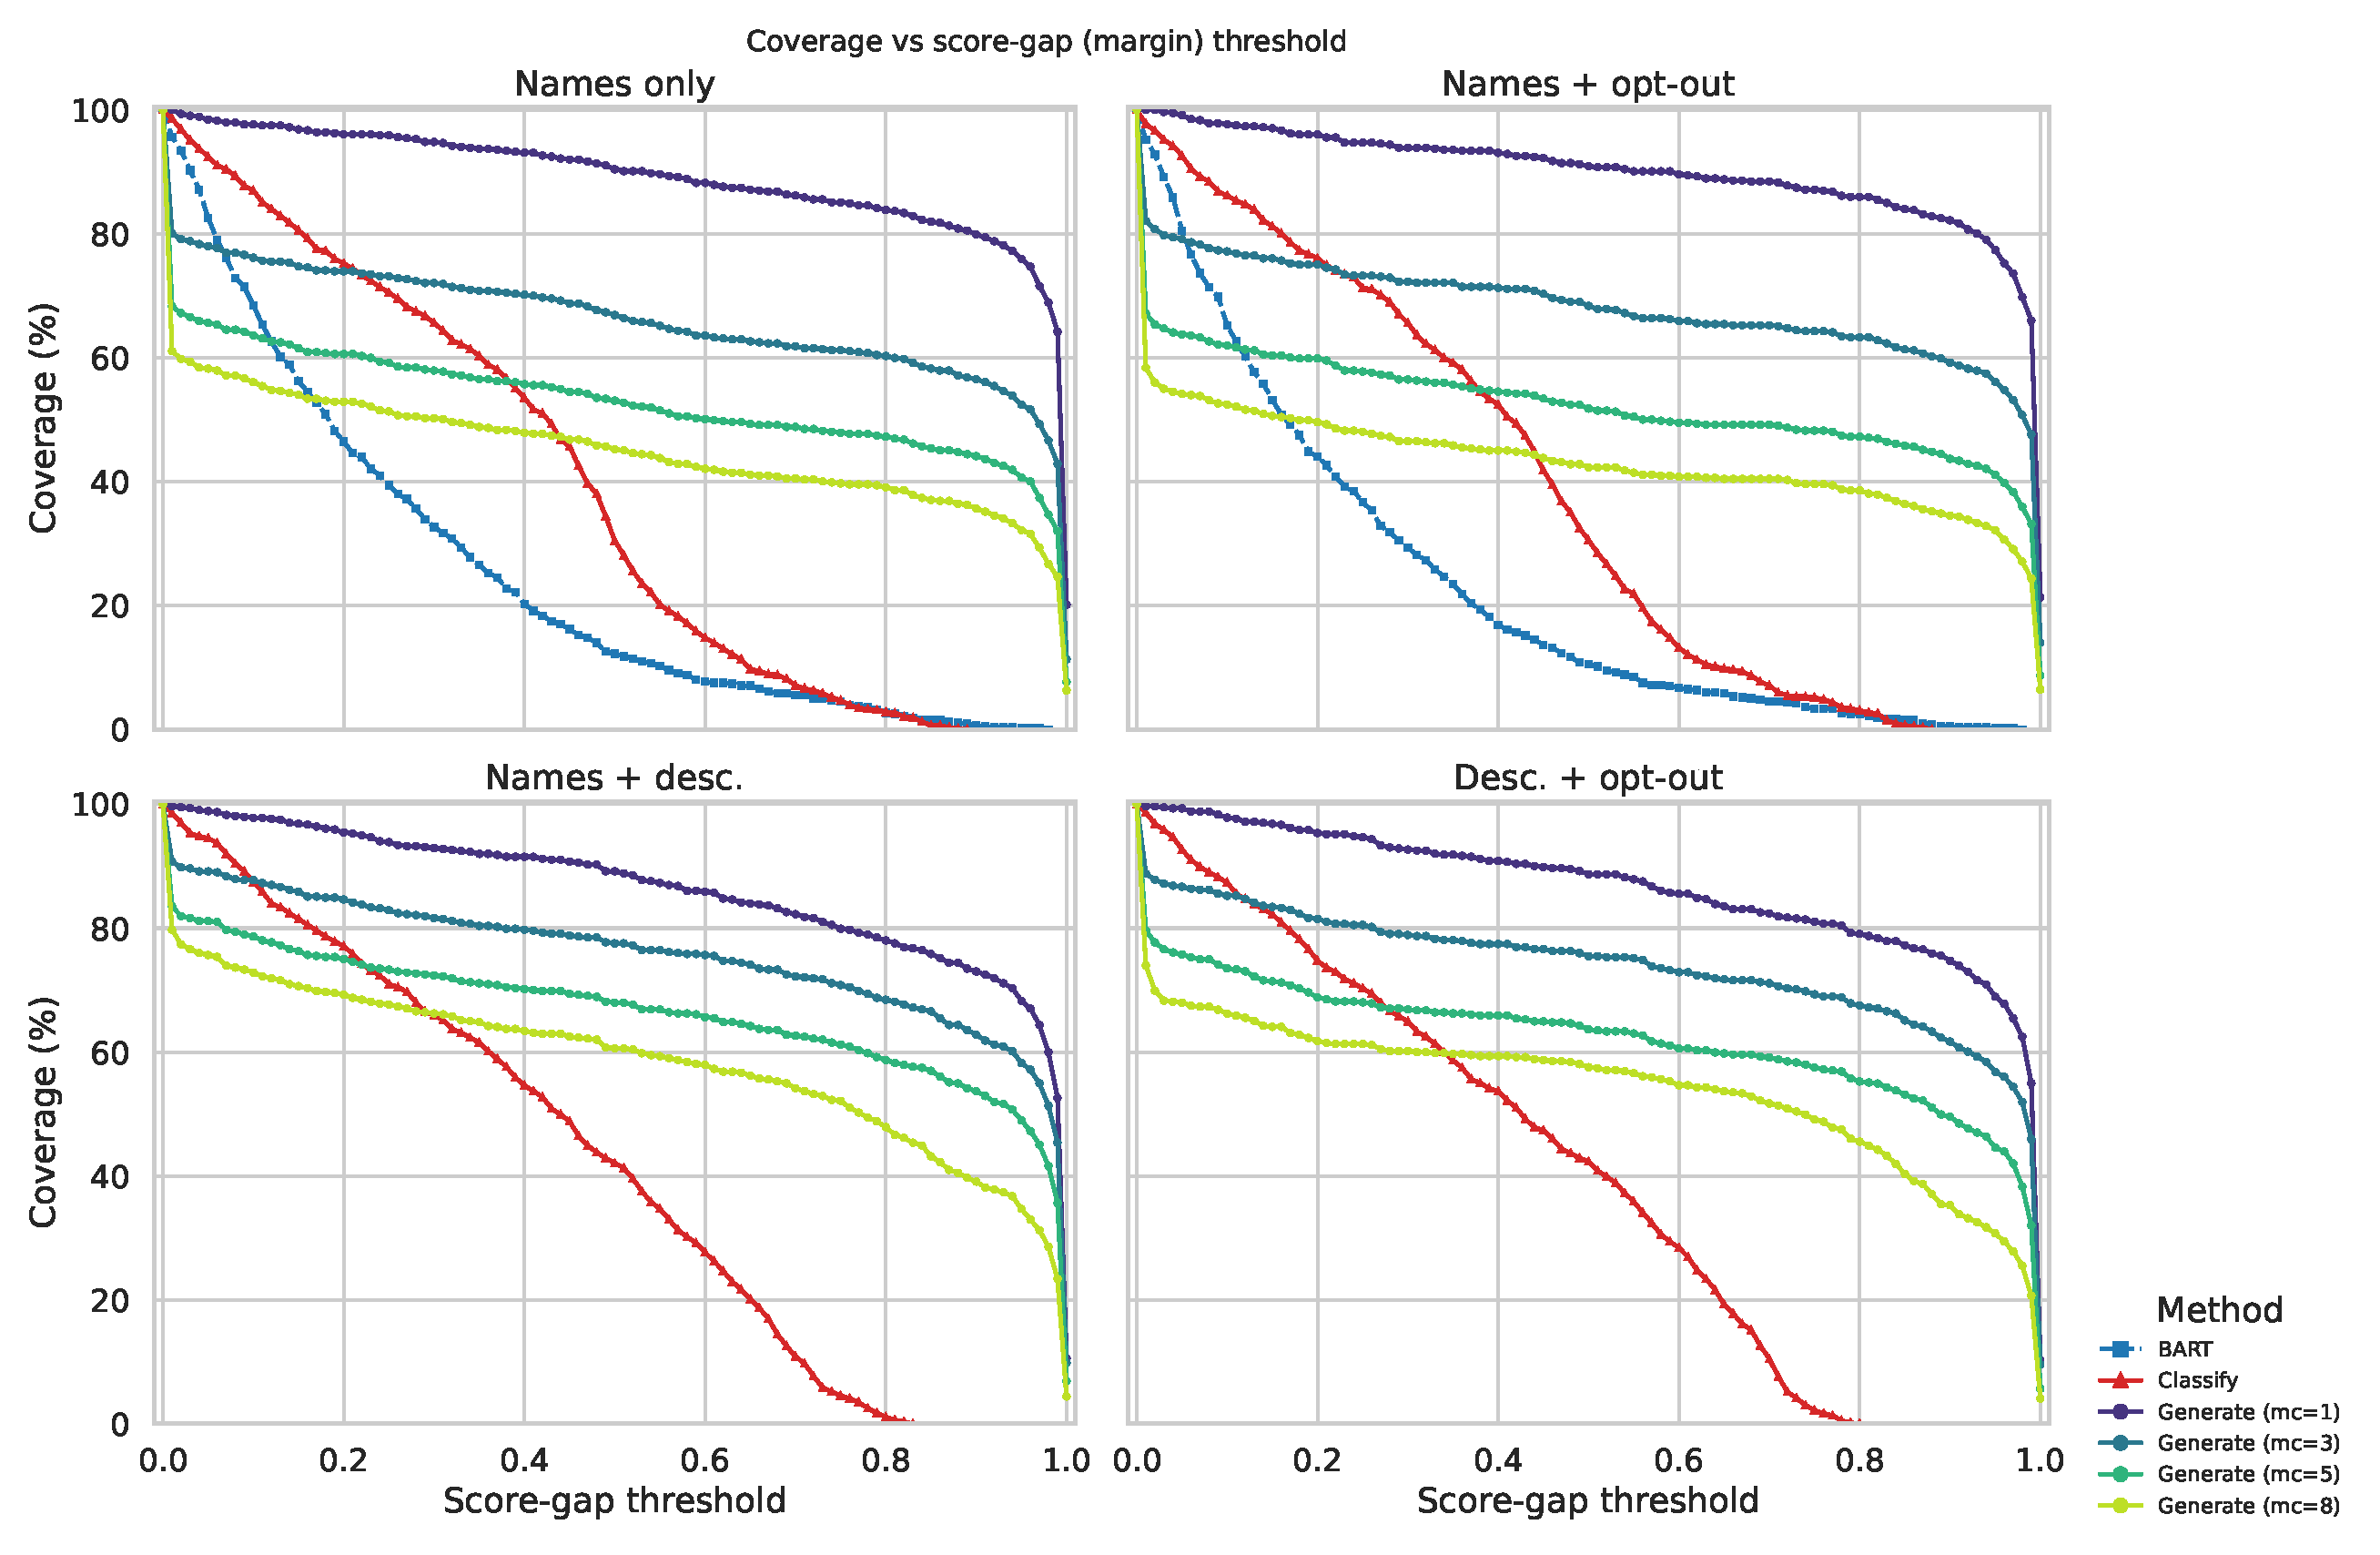
\includegraphics[width=\textwidth]{coverage_curve_margin}
    \caption{Coverage vs.\ score-gap threshold.}
    \label{fig:coverage-margin}
  \end{subfigure}
  \caption{Accuracy--coverage trade-off under thresholding on the score gap
           (margin between the two highest class probabilities). The margin
           discriminates correctness about as well as confidence for the
           generative methods, providing a complementary triage axis.}
  \label{fig:tradeoff-margin}
\end{figure}

\begin{figure}[htbp]
  \centering
  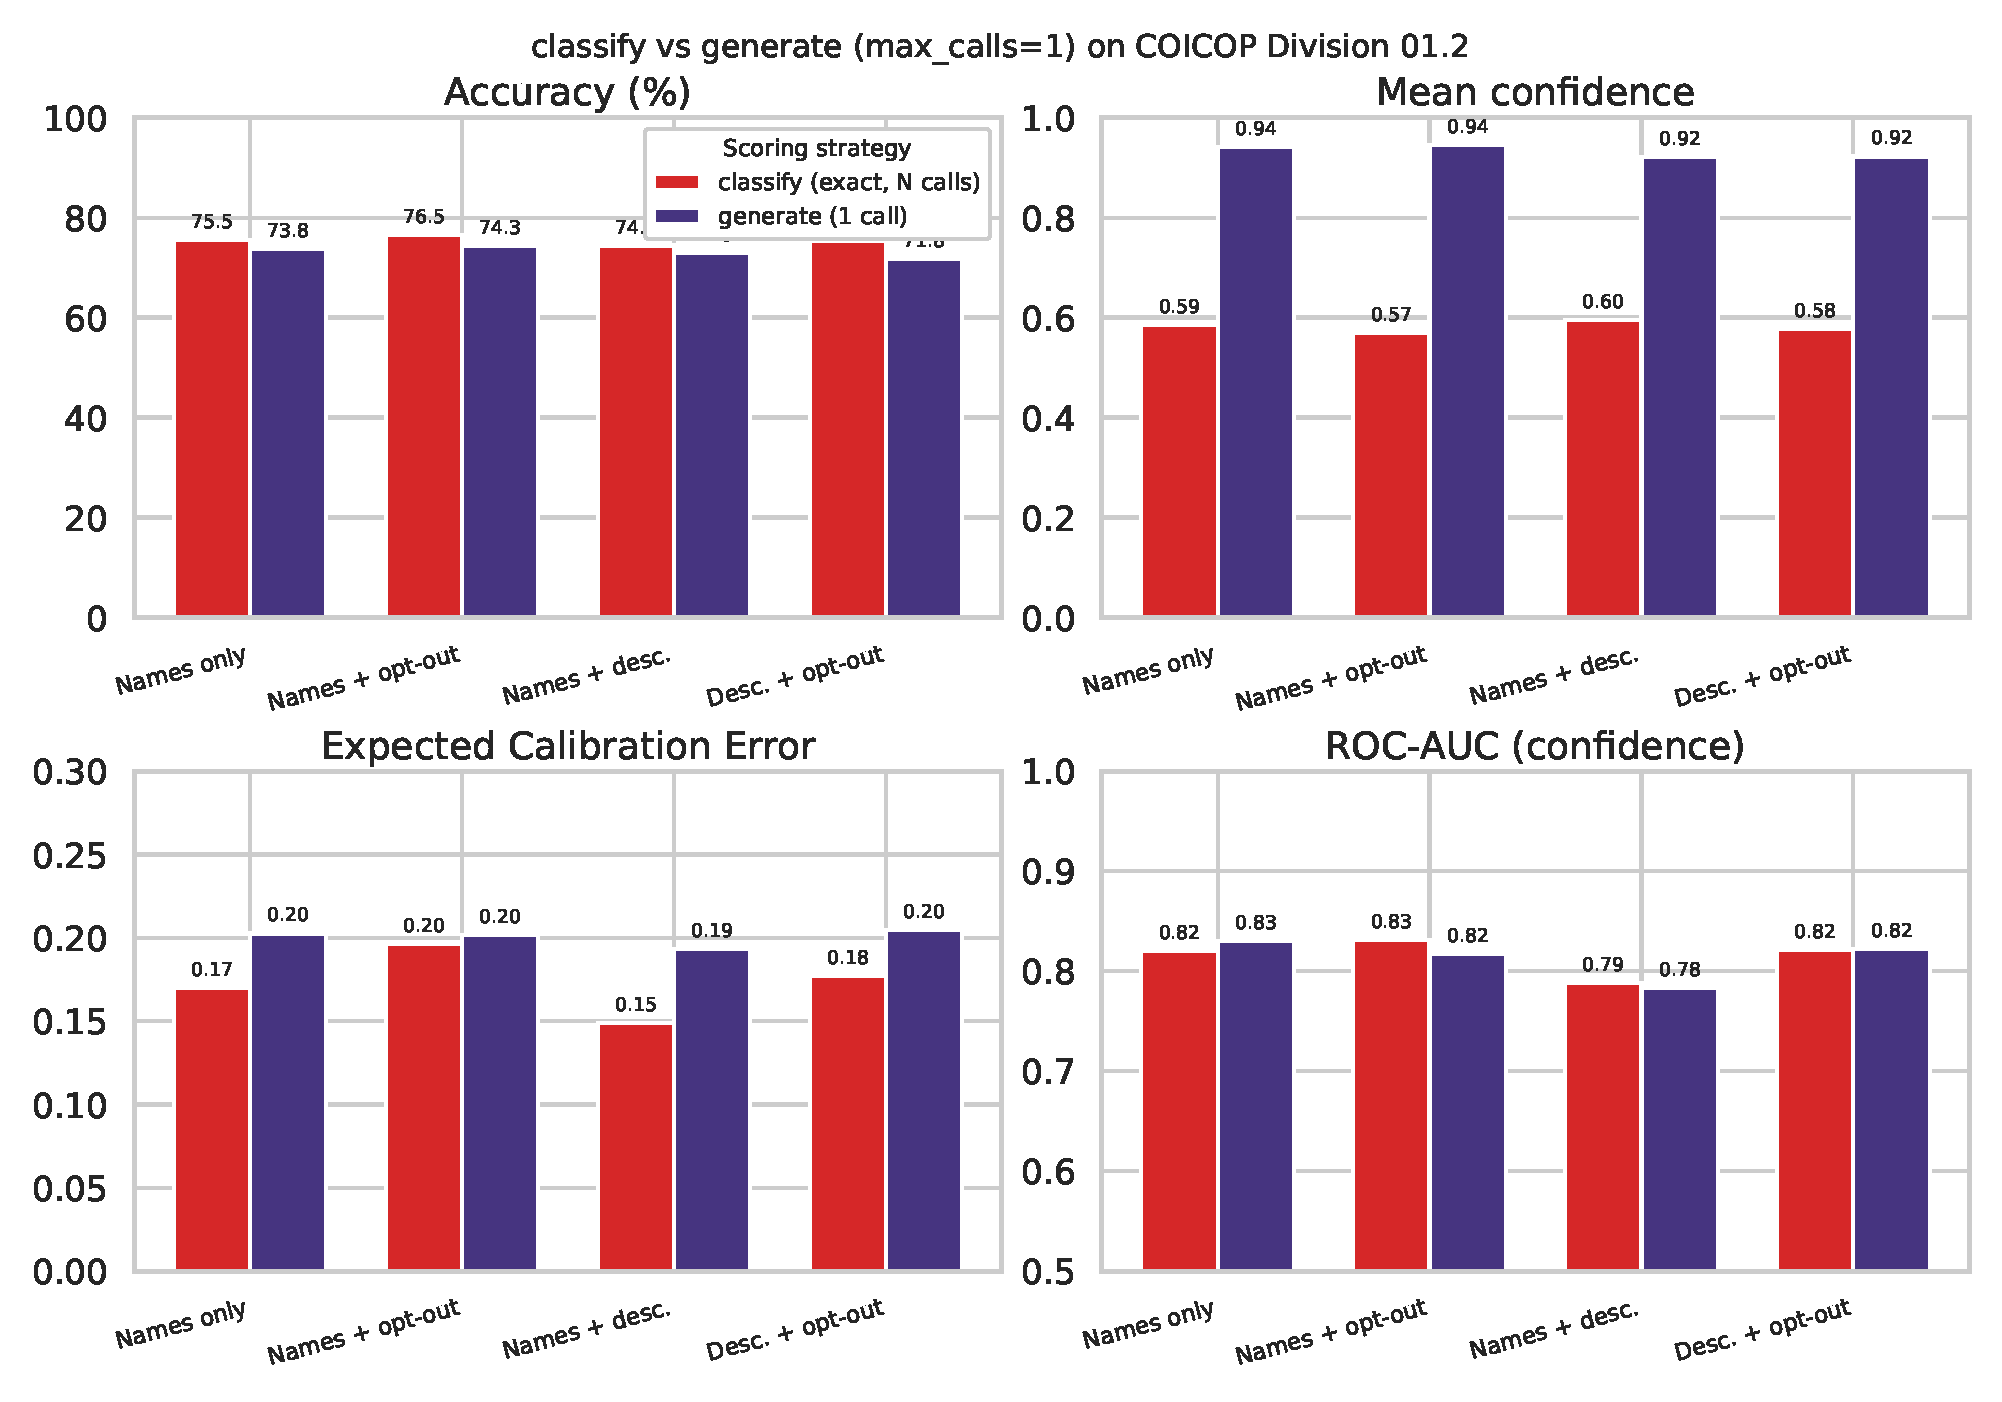
\includegraphics[width=0.9\textwidth]{generate_vs_classify}
  \caption{Generate (single call, \texttt{max\_calls}\,=\,1) vs.\
           \texttt{classify} (one call per label): accuracy, mean confidence,
           Expected Calibration Error, and ROC-AUC of confidence, by choice
           configuration. \texttt{generate} approaches \texttt{classify}
           accuracy at one-seventh to one-eighth the call cost (637 vs.\
           4{,}459--5{,}096 total calls) while returning a full probability
           distribution; it is markedly overconfident (higher ECE).}
  \label{fig:generate}
\end{figure}

\subsection{Limitations of the Evaluation}

Several caveats apply. The evaluation covers a single COICOP division (01.2),
and performance may differ where class boundaries are more ambiguous. We
evaluate one Ollama model (Qwen2.5 3B-Instruct); larger models may score
higher. The BART baseline runs on CPU, and GPU acceleration could narrow the
runtime gap. We do not include a fine-tuned classifier baseline, which would
require task-specific training data. Finally, because scikit-llm is
label-only, it is excluded from the confidence, calibration, and threshold
analyses.

% =============================================================================
\section{Discussion}
\label{sec:discussion}
% =============================================================================

\subsection{Design Decisions}

Three decisions distinguish \texttt{ollama-classifier}. First, it is
\emph{local-first}: defaulting to Ollama prioritizes privacy and
cost-effectiveness, while the vLLM, SGLang, and llama.cpp backends let users
match the engine to their hardware. Second, it deliberately avoids
fine-tuning, relying on prompting and retrieval; this maximizes flexibility
(models, classes, and domains change without retraining) at the cost of
task-specific accuracy. Third, it exposes two scoring strategies with an
explicit cost--accuracy trade-off: \texttt{classify} spends one call per label
for exact, calibrated probabilities, whereas \texttt{generate} reconstructs a
full probability distribution from a single constrained call and refines it,
when asked, through mass-preserving cluster reproportioning that can only
sharpen the distribution within a group---so accuracy is monotone
non-decreasing in the call budget, and partial coverage is always reported
through the \texttt{coverage} field.

\subsection{Limitations}

Classification quality ultimately depends on the underlying model, and models
below roughly 3B parameters struggle on complex taxonomies;
\citet{nunes2025rac} report that models with fewer than 1.5B parameters are
only marginally useful. LLM-based classification is also subject to
data-driven bias \citep{gallegos2024bias}, and deployers in sensitive settings
should audit for it \citep{yuan2026biasahead}. The multi-call \texttt{classify}
strategy trades computation for calibrated confidence and may be expensive for
very large label sets, where the budget-controlled \texttt{generate} strategy
is preferable. Our calibration results show that the generative strategies are miscalibrated
in opposite directions---\texttt{classify} is underconfident and
\texttt{generate} is overconfident (both high ECE)---while remaining strong
rankers (high AUC); practical deployment should therefore prefer ranking-based
triage (Section~\ref{sec:results}) or post-hoc calibration, noting that
\texttt{classify} and \texttt{generate} require opposite corrections
(sharpening vs.\ softening). Finally, the GUI is a single-user desktop application;
multi-user, server-based deployments are left to future work.

% =============================================================================
\section{Conclusion}
\label{sec:conclusion}
% =============================================================================

We have presented \texttt{ollama-classifier}, an open-source Python library
for zero-shot and few-shot text classification with locally-hosted LLMs. The
library provides two confidence-bearing scoring strategies---multi-call
completion scoring and hierarchical constrained generation with mass-preserving
cluster refinement---across four
inference backends, with constrained output generation, batch and asynchronous
APIs, and a retrieval-augmented pipeline. A desktop GUI and cross-language
ports in R (\texttt{rollama}) and Rust
(\texttt{ollama-classifier-rs}) extend the same API to non-programmers and to
other ecosystems. On a COICOP product-classification benchmark, a compact 3B
model served locally substantially outperforms a BART NLI baseline and matches
scikit-llm, while its confidence scores and score gaps---though miscalibrated
in absolute terms---reliably discriminate correct from incorrect predictions
and support effective threshold-based triage. Future work will tighten
calibration through temperature scaling and conformal prediction, broaden the
retrieval-augmented pipeline, and add a collaborative web interface.

% =============================================================================
% References
% =============================================================================
\printbibliography

\end{document}
